\documentclass[main.tex,fontsize=8pt,paper=a4,paper=portrait,DIV=calc,]{scrartcl}
% Document
\usepackage[T1]{fontenc}
\usepackage[dvipsnames]{xcolor}
\usepackage[nswissgerman,english]{babel}
\renewcommand{\familydefault}{\sfdefault}

% Format
\usepackage[top=5mm,bottom=1mm,left=5mm,right=5mm]{geometry}
%\setlength{\headheight}{\baselineskip}
%\setlength{\headsep}{0mm}

%\usepackage{scrlayer-scrpage}
%\clearpairofpagestyles
%\chead{{\bfseries\TITLE, \AUTHOR, \pagename~\thepage}}

%\addtokomafont{pagehead}{\upshape}

\usepackage{multicol}
\setlength{\columnsep}{2mm}
\setlength{\columnseprule}{0.1pt}

% Math
\usepackage{amsmath}
\usepackage{amssymb}
\usepackage{amsfonts}

% Code
\usepackage{fancyvrb, etoolbox, listings, xcolor}
%\usemintedstyle{bw}

%\newminted[shell]{bash}{
%fontsize=\footnotesize,
%fontfamily=tt,
%breaklines=true,
%frame=single,
%framerule=0.1pt,
%framesep=2mm,
%tabsize=2
%}
%\newminted{css}{
%breaklines=true,
%tabsize=4,
%autogobble=true,
%escapeinside=||,
%stripall=true,
%stripnl=true,
%}

    \definecolor{lightgray}{rgb}{0.95, 0.95, 0.95}
    \definecolor{darkgray}{rgb}{0.4, 0.4, 0.4}
    \definecolor{purple}{rgb}{0.65, 0.12, 0.82}
    \definecolor{ocherCode}{rgb}{1, 0.5, 0} % #FF7F00 -> rgb(239, 169, 0)
    \definecolor{blueCode}{rgb}{0, 0, 0.93} % #0000EE -> rgb(0, 0, 238)
    \definecolor{greenCode}{rgb}{0, 0.6, 0} % #009900 -> rgb(0, 153, 0)
    \definecolor{teal}{rgb}{0.0, 0.5, 0.5}

\lstdefinestyle{code}{
    identifierstyle=\color{black},
    keywordstyle=\color{blue}\bfseries\small,
    ndkeywordstyle=\color{greenCode}\bfseries\small,
    stringstyle=\color{ocherCode}\ttfamily\small,
    commentstyle=\color{teal}\ttfamily\textit\small,
    basicstyle=\ttfamily\small,
    breakatwhitespace=false,         
    breaklines=true,                 
    captionpos=b,                    
    keepspaces=true,                 
    showspaces=false,                
    showstringspaces=false,
    showtabs=false,                  
    tabsize=2,
    belowskip=-5pt
}



% Images
\usepackage{graphicx}
\newcommand{\pic}{\includegraphics[scale=0.3]}
\graphicspath{{Screenshots/}{../Screenshots}}
\makeatletter
\def\pictext#1#2{%
    \@ifnextchar[{%
    \pictext@iiiii{#1}{#2}%
    }{%
      \pictext@iiiii{#1}{#2}[0.5,0.4,0.3]% Default is 5
    }%
}
\def\pictext@iiiii#1#2[#3,#4,#5]{\begin{minipage}{#3\textwidth}\includegraphics[scale=#4]{#1}\end{minipage}\begin{minipage}{#5\textwidth}#2\end{minipage}}
\def\minipg#1#2{%
    \@ifnextchar[{%
    \minipg@iiii{#1}{#2}%
    }{%
      \minipg@iiii{#1}{#2}[0.3,0.6]% Default is 5
    }%
}
\def\minipg@iiii#1#2[#3,#4]{\vspace{0.8mm}\begin{minipage}{#3\textwidth}#1\end{minipage}\begin{minipage}{#4\textwidth}#2\end{minipage}{\vspace{0.8mm}}}
\makeatother

%\newenvironment{minty}[2]% environment name
%{% begin code
%  \begin{minipage}{#1}
%  \begin{minted}{#2}
%}%
%{% end code
%  \end{minted}
%  \end{minipage}
%  \end{minty}\ignorespacesafterend
%} 

% Smaller Lists
\usepackage{enumitem}
\setlist[itemize,enumerate]{leftmargin=3mm, labelindent=0mm, labelwidth=1mm, labelsep=1mm, nosep}
\setlist[description]{leftmargin=0mm, nosep}
\setlength{\parindent}{0cm}

% Smaller Titles
\usepackage[explicit]{titlesec}

%% Color Boxes
\newcommand{\sectioncolor}[1]{\colorbox{black!60}{\parbox{0.989\linewidth}{\color{white}#1}}}
\newcommand{\subsectioncolor}[1]{\colorbox{black!50}{\parbox{0.989\linewidth}{\color{white}#1}}}
\newcommand{\subsubsectioncolor}[1]{\colorbox{black!40}{\parbox{0.989\linewidth}{\color{white}#1}}}
\newcommand{\paragraphcolor}[1]{\colorbox{black!30}{\parbox{0.989\linewidth}{\color{white}#1}}}
\newcommand{\subparagraphcolor}[1]{\colorbox{black!20}{\parbox{0.989\linewidth}{\color{white}#1}}}

%% Title Format
\titleformat{\section}{\vspace{0.5mm}\bfseries}{}{0mm}{\sectioncolor{\thesection~#1}}[{\vspace{0.5mm}}]
\titleformat{\subsection}{\vspace{0.5mm}\bfseries}{}{0mm}{\subsectioncolor{\thesubsection~#1}}[{\vspace{0.5mm}}]
\titleformat{\subsubsection}{\vspace{0.5mm}\bfseries}{}{0mm}{\subsubsectioncolor{\thesubsubsection~#1}}[{\vspace{0.5mm}}]
\titleformat{\paragraph}{\vspace{0.5mm}\bfseries}{}{0mm}{\paragraphcolor{\theparagraph~#1}}[{\vspace{0.5mm}}]
\titleformat{\subparagraph}{\vspace{0.5mm}\bfseries}{}{0mm}{\subparagraphcolor{\thesubparagraph~#1}}[{\vspace{0.5mm}}]

%% Title Spacing
\titlespacing{\section}{0mm}{0mm}{0mm}
\titlespacing{\subsection}{0mm}{0mm}{0mm}
\titlespacing{\subsubsection}{0mm}{0mm}{0mm}
\titlespacing{\paragraph}{0mm}{0mm}{0mm}
\titlespacing{\subparagraph}{0mm}{0mm}{0mm}

%% format cells
\usepackage[document]{ragged2e}
\usepackage{array, makecell}
\renewcommand{\arraystretch}{2}
\newcommand{\mc}{\makecell[{{m{1\linewidth}}}]}


\usepackage{listings-rust}

\lstset{
    language=Rust,
    style=colouredRust,
}
%%%%%

\begin{document}
\begin{table}[h!]
\section{Cargo}
\begin{tabular}{|m{0.2\linewidth}|m{0.755\linewidth}|}
\hline
Default Commands &
\vspace{2mm}
\begin{itemize}
  \item \textcolor{teal}{Cargo new} creates a new rust project with git integration
  \item \textcolor{teal}{Cargo build} build a project if the toml file has been provided
  \item \textcolor{teal}{Cargo build --release} builds the release version without debugging environment
  \item \textcolor{teal}{Cargo run} runs the project
  \item \textcolor{teal}{Cargo check} this only checks the code if it would compile! But it doesn't actually compile! Super helpful!
  \vspace{-3mm}
\end{itemize}\\
\hline
Toml & 
\begin{lstlisting}
[package]
name = "hello_cargo"
version = "0.1.0"
edition = "2021"

[dependencies]
\end{lstlisting}
\\
\hline
\end{tabular}
\section{Basic Terms and Information}
\begin{tabular}{|m{0.2\linewidth}|m{0.755\linewidth}|}
\hline
Comments & 
\textcolor{orange}{Comments are made with // just like C++ or C}\\
\hline
Main & 
\textcolor{orange}{Just like c++, the first function is always main!}\newline
\textcolor{teal}{However, unlike c++ the function definition order doesn't matter, there is no need for hpp files or similar!}\newline
\textcolor{purple}{The function main always needs to return either 0 -> () or -> Result<(), E> (this type is explained further below in error handling).}\newline
\textcolor{purple}{the underlying convention of Result<(), E> is either return 0 aka () if ok, or return some other integer in case of error\newline
You can however also return other types, that implement the "std::process::Termination" trait (also explained later)}\\
\hline
Naming convention & 
\vspace{2mm}
\begin{itemize}
  \item \textcolor{teal}{Functions: some\_function\_name()}
  \item \textcolor{teal}{}
  \item \textcolor{teal}{}
  \item \textcolor{teal}{}
  \vspace{-3mm}
\end{itemize}\\
\hline
\textbf{Macros} & 
\textcolor{orange}{You use a macro with the "!" keyword after a function}\newline
\begin{lstlisting}
fn main() {
    println!("Henlo birb!");
}
\end{lstlisting}\\
\hline
Variable definition & 
\textcolor{orange}{Rust has a peculiar syntax for writing variables, it is very much different to all other languages}\newline
\begin{lstlisting}
let num = 5; 
// this produces an immutable variable num, yes IMMUTABLE!!

let mut num2 = 5;
// num2 is MUTABLE because of the mut keyword!!

let mut num3: u32 = 5;
// this specifies a type of u32 int to the variable!
\end{lstlisting}\\
\hline
Strings & 
\textcolor{orange}{Strings in rust are strange, they are declared as follows:}\newline
\begin{lstlisting}
let mut grief = String::new();
// empty string

let mut grief = String::from("grief");
// mutable string with value "grief"
\end{lstlisting}
\, \newline
\textcolor{teal}{However, there are also trivial strings, they just do not have all the functions of the other strings.\newline
They do however in contrast work just like regular strings in c++.}\newline
\begin{lstlisting}
let mut str = "ping";
println!("{str}"); //prints ping
str += "pang";
println!("{str}"); //prints pingpang
\end{lstlisting}\\
\hline
\end{tabular}
\end{table}
\pagebreak
\begin{table}[ht!]
\begin{tabular}{|m{0.2\linewidth}|m{0.755\linewidth}|}
\hline
Input \& Output & 
\begin{lstlisting}
std::io::stdin()
         .read_line(&mut num2)
         .expect("Failed to read line");
// the &mut is needed to reference the num2 variable as a mutable reference
// This string has by default an added newline,
// to get rid of this we have to format it
let num2 = num2.trim();
// this will create a new num2 variable and ghost the last one!!!
// .trim() will remove all whitespaces at the front and at the back
// just like definition it is by default immutable
// expect will trigger if the input has failed

// interesting is also the printing of variables inside println!
println!("The number is {num2}")
println!("The number is {},num2")
// these are identical! 
// If you have multiple numbers you have to order them in the same way as the empty {} are.
\end{lstlisting}
\, \newline
\textcolor{orange}{Similar to C++ we need namespaces to use standard library functions}\newline
\textcolor{teal}{.read\_line() has a result of either "Ok", or "Err" which must be handled with the .expected() function! \newline
This apparently will (guess) throw an error}\\
\hline
\end{tabular}
\end{table}
\pagebreak
\begin{table}[ht!]
\begin{tabular}{|m{0.2\linewidth}|m{0.755\linewidth}|}
\hline
conditional on Input & 
\textcolor{orange}{Instead of just parsing a string,\newline
we can also use functions on fail or ok states!}\newline
\begin{lstlisting}
loop {
    let mut guess = String::new();
    std::io::stdin()
        .read_line(&mut guess)
        .expect("failed to read line")
    
    let guess: u32 = match guess.trim().parse() { // match the parsed string
        Ok(num) => num, // if the string is a u32 int, then create the var num with that value
        Err(_) => continue, // continue the loop if it is not a u32 int
    }

}
\end{lstlisting}\\
\hline
loops & 
\textcolor{orange}{The easiest but also silliest loop in rust is the simple keyword: \textbf{loop}, it creates an infinite loop!}\newline
\begin{lstlisting}
loop {
    println!("I will print ping pang until you close the program!");
}
\end{lstlisting}\\
\hline
comparisons & 
\textcolor{orange}{Rust allows for a strange comparison syntax:}\newline
\begin{lstlisting}
loop {
    match guess.cmp(&secret_number) {
        Ordering::Less => println!("Too small!"), // do if guess is smaller
        Ordering::Greater => println!("Too big!"), // do if guess is bigger
        Ordering::Equal => { // do if guess is same!
            println!("You win!");
            break; // break loop
        }
    }
}
// Theoretically this is the same as a bunch of if-statements,
// however, I have no idea how the performance compapres....
\end{lstlisting}\\
\hline
random numbers & 
\textcolor{orange}{Unlike C or C++ you do not need to provide a seed.\newline
Just like in python you can simply use the rand function:}\newline
\begin{lstlisting}
let secret_number = rand::Rng::treadh_rng().gen_range(1..=100);
// this creates a rnadom number with range 1 to and with 100.
\end{lstlisting}\\
\hline
Constants & 
\begin{lstlisting}
cont SOME_CONSTANT: u32 = 5;
\end{lstlisting}\\
\hline
Scopes and Shadowing & 
\textcolor{orange}{Just like c++, when we have scopes and we redefine a variable, then it will only overwrite said variable in that scope.}\newline 
\begin{lstlisting}
let x = 5;
{ // empty scope
    let x = 10;
    println!({&x});
    // prints 10
}
println!({$x});
// prints 5
\end{lstlisting}
\, \newline
\textcolor{teal}{Interesting to know, you can create another variable with a different type and the same name!\newline 
This will still just shadow the previous one, \textbf{HOWEVER}, }\textcolor{red}{Shadowing does \textbf{NOT work with mutable variables!}}\newline
\begin{lstlisting}
let x = 5;
let x = "ping";
// OK
let mut y = 5;
let mut y = "ping";
// ERROR! can't shadow mutable variable
\end{lstlisting}\\
\hline 
Integer Sizes& 
\vspace{2mm}
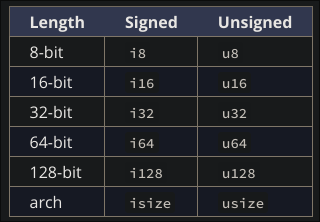
\includegraphics[scale=0.45]{2022-10-19-01:21:45.png}
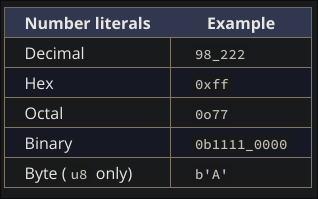
\includegraphics[scale=0.45]{2022-10-19-01:25:19.png}\newline
\textcolor{orange}{The default is i32 integer}
\\
\hline
\end{tabular}
\end{table}
\pagebreak
\begin{table}[ht!]
\begin{tabular}{|m{0.2\linewidth}|m{0.755\linewidth}|}
\hline
Float and double & 
\textcolor{orange}{In rust double is the default floating point type!}\newline
\begin{lstlisting}
let x = 5.5; // has type f64 -> double
let x: f32 = 5.5; // this is a float -> float is f32
\end{lstlisting}
\, \newline 
\textcolor{teal}{Note for calculations, just like in c++ if you do divisions,
make sure you use floats, unless you want truncated values:}\newline
\begin{lstlisting}
let x = 5 / 2;
// x = 2!
let x = 5.0 / 2.0;
// x = 2.5
\end{lstlisting}
\\
\hline
Chars & 
\begin{lstlisting}
fn main() {
    let c = 'z';
    let z: char = 'Z'; // with explicit type annotation
    let heart_eyed_cat = 'emoj';
    // latex might not show it, but you can insert emojis....
}
\end{lstlisting}\\
\hline
Tuples & 
\textcolor{orange}{Tuples are very easy in rust!}\newline
\begin{lstlisting}
    // creating a tuple
    let tup: (i32, f64, u8) = (500, 6.4, 1);

    //accessing a tuple
    let num = tup.1;
    // assigns the first value of tup -> num = 500
    // tup.2 -> 6.4, tup.3 -> 1

    let tup2 = (500, 6.4, 1);
    let (x, y, z) = tup2;
    // assign x = 500, y = 6.4, z = 1
\end{lstlisting}\\
\hline
Arrays & 
\begin{lstlisting}
// creating arrays
let arr = [1,2,3,4,5];
// implicit type and size
let arr2: [i32;5] = [1,2,3,4,5];
// explicit type and size
let arr3 = [3;5];
// creates an array of: [3,3,3,3,3] 5 times the value 3

// accessing arrays -> done just like c++
// arr[0] -> 1
// arr[1] -> 2
// should you go out of bounds, it will panick -> runtime error
\end{lstlisting}\\
\hline
Function Parameters &
\textcolor{orange}{Function parameters are always explicit!}\newline
\begin{lstlisting}
fn some_func(x: i32, y: char) {
    println!("value of {y} is {x}");
}
some_func(5,'h');
\end{lstlisting}\\
\hline
Scopes in rust & 
\begin{lstlisting}
let y = {
        let x = 3;
        x + 1 // no error this works because of the scope!
    }; // it's essentially a return statement!

println!("The value of y is: {y}");
// will print the value 4
\end{lstlisting}\\
\hline
\textbf{Return} & 
\textcolor{orange}{\textbf{In Rust functions can return values implicitly, and it is also used like this!}}\newline
\begin{lstlisting}
fn ret() -> i32 { // you must specify the return like this! i32 for int
    5
}
// this function simply returns 5 !!
fn ret2() -> (i32, String) {
    (5, "henlo birb!") // Rust allows you to return tuples as well!!
}
\end{lstlisting}
\, \newline
\textcolor{teal}{You can still use the return keyword in rust, it is just not needed -> choose a style...}\newline
\textcolor{red}{\textbf{More importantly: the return value MUST be written and it is after an arrow: \emph{->}}}\\
\hline
\end{tabular}
\end{table}
\pagebreak
\begin{table}[ht!]
\begin{tabular}{|m{0.2\linewidth}|m{0.755\linewidth}|}
\hline
Expressions vs Statements &
\textcolor{red}{\textbf{VERY IMPORTANT, rust makes a clear difference between an expression and a statement.}}\newline
\textcolor{orange}{A statement is something like a variable to return in a function, while an expression is something like a function call some\_func()}\newline
\textcolor{red}{\textbf{So, yes, when returning a value you do not put a semicolon at the end!}}\newline
\begin{lstlisting}
fn some_func() -> i32 {
    5 // NO SEMICOLON!!!!!
    5; // WRONG!!!!
}
\end{lstlisting}\\
\hline
If statements & 
\textcolor{orange}{In rust if statements do not need brackets around them, the compiler even tells you about unnecessary brackets!}\newline
\begin{lstlisting}
if x > 5 {
    println!("ping pang");
} else {
    println!("sadly no pang ping");
}
\end{lstlisting}
\, \newline
\textcolor{teal}{There is one more caviat, since rust does not do implicit type conversion if there is data loss, it also doesn't convert integers to booleans!}
\begin{lstlisting}
let x = 5;
if x {
 // doesn't work !!! error implicit cast not allowed!
}
if x != 0 {
 // works
}
\end{lstlisting}\\
\hline
Inline If & 
\textcolor{teal}{You can also write inline if statements to for example assign a value to a variable:}\newline
\begin{lstlisting}
let x = 5;
let y = if x > 6 {4} else {3};
// y now has the value of 3 as x is not greater than 6
\end{lstlisting}\\
\hline
Loops & 
\textcolor{orange}{Prepare for brainfuck, loops in rust are super weird, here an example with comparison to c++}\newline
\textcolor{teal}{Note that this can be done differently with a for loop in c++!}\newline
\begin{lstlisting}
fn main() {                                    void main() {        
    let mut counter = 0;                           int result = 0;
                                                   int counter = 0;
    let result = loop {                            while (true) {
        counter += 1;                                  if (counter == 10) { 
                                                          result = counter * 2;
        if counter == 10 {                             } 
            break counter * 2;                     counter += 1;
        // <<< result = counter * 2 !!!!          }
        }                                      std::cout << "The result is " << result << "\n";
    };                                         }
    println!("The result is {result}");       
}
\end{lstlisting}
\, \newline
\textcolor{orange}{Take a close look at the break counter * 2, this is essentially a return statement from a loop that will be assigned to the variable result.}\\
\hline
Loops with labels &
\textcolor{orange}{Another quirk with loops in rust is that you can assign labels to loops, this is needed to break out of a loop without assigning a value!}\newline
\begin{lstlisting}
let mut counter = 0;
'some_name: loop { // notice the ' at the start !!!!
    if counter == 2 {
        break 'some_name; // break the loop with label some_name
        // this means you can break loops nested loops!!!!
    }
    counter += 1;
}
\end{lstlisting}\\
\hline
While Loops &
\textcolor{teal}{While loops are the same as c++ without the brackets.}\newline
\begin{lstlisting}
let mut counter = 0;
while counter != 3 {
    counter += 1;
    println!({counter});
}
\end{lstlisting}\\
\hline
\end{tabular}
\end{table}
\pagebreak
\begin{table}[ht!]
\begin{tabular}{|m{0.2\linewidth}|m{0.755\linewidth}|}
\hline
For Loops &
\textcolor{teal}{For loops can be used like ranged based for loops in c++ and co.}\newline
\begin{lstlisting}
let x = [1,2,3,4,5];
for element in x {
    println!({element});
}
\end{lstlisting}
\, \newline
\textcolor{orange}{For loops like this for (int i = 0; i < x.size; i++), you write the following:}\newline
\begin{lstlisting}
for number in (1..x.size()).rev() { // x.size == 4
    // instead of x.size you can put any number there !
    println!("{number}!");
}
\end{lstlisting}\\
\hline
\textbf{\textcolor{red}{Ownership}} & 
\textcolor{orange}{This is the reason you use rust, it is the management of ownership that makes rust both safe and fast. It is a third approach to memory handling next to the known garbage collector system and the raw pointer approach from c and c++}\newline
\textcolor{teal}{The ownership system states, that each heap value must always have an owner, if this requirement is not fulfilled, then the value will be dropped.\newline
This can be compared to a pointer in c++ with the only difference being the fact that the value in c++ can have no pointer as well -> PROBABLE MEMORY LEAK!}\newline
\textcolor{red}{Here is a list of rules that you must follow when programming in rust:} \newline
\begin{enumerate}
\item \textcolor{teal}{\textbf{Each heap value must ALWAYS have an owner}}
\item \textcolor{teal}{\textbf{Each heap value can only have 1 owner at a time}}
\item \textcolor{teal}{\textbf{The owner can change!}}
\item \textcolor{teal}{\textbf{If a value loses it's owner without a replacement, the value will be dropped -> deleted from memory}}
\vspace{-3mm}
\end{enumerate}
\\
\hline
Heap allocated variables & 
\textcolor{orange}{In rust heap allocated variables are essentially just pointers, similar to how java handles them, however, unlike java, rust only allows 1 variable to reference the heap.\newline
As already stated above, only 1 owner may be present at any time.\newline
This result in the following scenario:}\newline
\begin{lstlisting}
    let s1 = String::from("hello"); // declare the heap allocated string s1
    let s2 = s1; // declare s2 with the values at the memory address s1 points to
                 // ownership is transfered to s2! therefore >>s1 IS OUT OF SCOPE<<
    println!("{}, world!", s1); // ERROR s1 is dropped, aka it is no longer defined!
\end{lstlisting}
\, \newline
\textcolor{red}{This behavior not only makes sense, it also enforces move semantics, as you can't make endless copies of pointers that are unnecessary! \newline
But it also makes sure that you don't make copies implicitly with new constructors!}\\
\hline
Copying Heap variables & 
\textcolor{orange}{Of course, you can still copy the data of heap allocated variables should you wish to have it this way, however, you need to explicitly call a clone function to do this!}\newline
\begin{lstlisting}
let s1 = String::from("hello"); // allocate s1 from heap
let s2 = s1.clone(); // copy data from s1 and allocate s2 from heap

println!("s1 = {}, s2 = {}", s1, s2); // both are valid!
\end{lstlisting}\\
\hline 
Copy only Types & 
\textcolor{orange}{Just like java, there are type that can't be represented by a reference/pointer, so called Copy only types.\newline
However, unlike java this is not to take away control, but to remove unnecessary overhead on types that are faster when used on the stack\newline}
\textcolor{red}{\textbf{All types that have a known size at compile time are copy types!}}\newline
\begin{lstlisting}
let x = 5;
let y = x;

println!("{x}{y}"); // both variables valid as integer is a copy type!
\end{lstlisting}
\, \newline
\textcolor{orange}{User defined Types can implement the \textbf{Copy} trait, this specifies that this type is of known size on compile time, and can therefore be used on the stack!}\newline
\textcolor{orange}{On the same note, there is the \textbf{Drop} trait which specifies the opposite, they are \textbf{mutually exclusive}!}\\
\hline
List of Copy/Drop types & \minipg{
\textcolor{green}{Copy Types}\newline
\begin{itemize}
\item Integers -> i32, i64, u32, u64
\item Booleans -> true, false
\item Float -> f32, f64
\item Chars -> 'a','b','c',...
\item Tuples! \textcolor{teal}{if they contain only Copy elements}
\end{itemize}}
{\textcolor{red}{Drop Types:}\newline
EVERYTHING ELSE!\newline
\, \newline
\, \newline
\, \newline
\, \newline
}[0.4,0.4]\\ 
\hline
\end{tabular}
\end{table}
\pagebreak 
\begin{table}[ht!]
\begin{tabular}{|m{0.2\linewidth}|m{0.755\linewidth}|}
\hline
Functions and Heap variables & 
\textcolor{orange}{Just like when defining a new variable with existing data from heap, when passing a heap allocated variable, you will find that your original variable has been dropped, which means you either have to use a new one, or take ownership back from said function when done.}\newline
\begin{lstlisting}
fn ping() {
let x = String::from("pingpang!");
some_func(x);
// x out of scope!!!!!
println!("{x}"); // error, x no longer defined! -> droppped
}

fn some_func(x: String) {
println!("{x}"); // works
}
\end{lstlisting}\\
\hline
Ownership changes & 
\textcolor{orange}{Just like we move the ownership to a function by passing it as a parameter, the function can pass it back instead of dropping the value.\newline
This can simply be done by returning the variable in question and then assigning it to either a new variable in the originating function, or taking the old variable that no longer had ownership -> redefining it}\newline
\begin{lstlisting}
fn ping() {
let x = String::from("ping!");

let y = pang(x);

println!("{x}"); // error as expected!
println!("{y}"); // works as y is now in scope with the returned x from pang()!!
}

fn pang(x: String) -> String {
    x
}
\end{lstlisting}\\
\hline
References & 
\textcolor{orange}{References in rust are used to manipulate/use variables without taking ownership of them. \newline
This means that we can pass a reference to a function and the variable to that reference is still valid. \newline
All we essentially do is create a pointer to a pointer.}\newline
\begin{lstlisting}
fn ping() {
    let x = String::from("ping");
    pang(&x); // call pang with reference of x
    println!("{x}"); // still valid as x was only a reference
}

fn pang(x: String) {
    println!("{x}"); // obviously valid
}
\end{lstlisting}
\, \newline
\textcolor{teal}{The act of creating references in rust is called \textbf{Borrowing}.}\newline
\textcolor{red}{Note that just like variables, a reference is also immutable by default!}\\
\hline
Immutable vs Mutable References & 
\textcolor{red}{There is one big difference between mutable and immutable references other than the mutability, namely the amount of them that can exist.\newline
\textbf{There can be an infinite amount of immutable references to a value, but only ONE mutable one!}\newline
This restriction guarantees, that there will be no undefined behavior due to changes from other mutations -> multithreading}
\, \newline
\, \newline
\begin{itemize}
\item \large \textcolor{red}{Only 1 mutable reference at a time}
\item \large \textcolor{red}{Infinite amount of immutable reference at a time}
\item \large \textcolor{red}{Combining both is not allowed!! Either x amount of immutable or 1 mutable!}
\end{itemize}
\normalsize \, \newline
\begin{lstlisting}
{
    let x = 5;
    let a = &x; // ok 1. immutable reference
    let b = &x; // ok 2. immutable reference
    let c = &mut x; // ERROR mutable and immutable references at the same time!
}
{
    let x = 5;
    let a = &mut x; // ok 1. mutable reference
    let b = &mut x; // ERROR no more than 1 mutable reference allowed
    let c = &x; // ERROR mutable and immutable references at the same time!
}
\end{lstlisting}
\, \newline
\textcolor{teal}{Hint, just like other variables, references go out of scope, use this to your advantage -> create another mutable reference when the last one goes out of scope.}\\
\hline
\end{tabular}
\end{table}
\pagebreak
\begin{table}[ht!]
\begin{tabular}{|m{0.2\linewidth}|m{0.755\linewidth}|}
\hline
Non-Lexical Lifetimes(NLL) & 
\textcolor{orange}{This concept defines that a variable can go out of scope before the end of a scope, this means that it will vanish somewhere in the middle of (for example) a function.\newline
Rust utilizes this in order to allow for more flexibility when using both mutable and immutable references after each other!\newline
The compiler will check if the variable is going to be used again and if not, the code will compile. Here an example:}\newline
\begin{lstlisting}
let mut x = String::from("pingpang");
let a = &x; // ok
println!("{a}");
// the reference a will no longer be used from here on -> out of scope!!

let b = &mut x; // ok
println!("{b}");
\end{lstlisting}\\
\hline
Nullpointers & 
\textcolor{orange}{Simple, they \textbf{don't exist in rust}.}\newline
\begin{lstlisting}
fn main() {
    let reference_to_nothing = dangle();
}

fn dangle() -> &String {
    let s = String::from("hello");

    &s // we try to return a reference to s, but s is going out of scope in the next line
       // this would not compile!! memory of s is freed here!
       // small note there is a feature called lifetime borrowing that would allow this
       // will be covered later
}
\end{lstlisting}
\, \newline
\textcolor{teal}{The dropping mechanism also has another aspect, all references will be out of scope if the underlying memory is dropped, as there may be no reference to nullptr!!}\\
\hline
String Slices & 
\textcolor{orange}{Consider the following scenario, if you want to know the size of the first word in a string, then you have to iterate over this string and return the integer. This is at least how it worked for other languages, and it is also possible in rust:}\newline
\begin{lstlisting}
fn first_word(s: &String) -> usize {
    let bytes = s.as_bytes(); // turn the string to bytes
    for (i, &item) in bytes.iter().enumerate() { // iterate over the bytes 
        if item == b' ' { // it gives us both the reference item and the iterator i
            return i; // return i if we find whitespace -> b' ' is the bytewhitespace
        }
    }
    s.len() // return the string length otherwise
}
\end{lstlisting}
\, \newline
\textcolor{orange}{This code looks like it works, and it also compiles, however it has a major flaw, as soon as we change the string that we entered, the size of the first word is useless! }\newline
\begin{lstlisting}
fn main() {
    let mut s = String::from("hello world");
    let word = first_word(&s); // word will get the value 5
    s.clear(); // this empties the String, making it equal to ""
    // word still has the value 5 here, but there's no more string that
    // we could meaningfully use the value 5 with. word is now totally invalid!
}
\end{lstlisting}
\, \newline
\textcolor{orange}{Rust has a very neat way to address this issue called String Slices, with it you can reference a part of a string. Yes, you heard that right, you can reference A PART of a string!!}\newline
\begin{lstlisting}
let s = String::from("hello world");

let hello = &s[0..5]; // references hello
// let hello = &s[..5] is the same, the 0 at the start can be omitted
let world = &s[6..11]; // references world
// let world = &s[6..] is the same as the end index would be the end of the string
// let s2 = &s[..] this would simply be the entire string
// &s[starting_index .. ending_index]
\end{lstlisting}
\, \newline
\textcolor{orange}{With this information in mind, we can now return a reference to the first word instead of the length of it.}\newline
\begin{lstlisting}
fn first_word(s: &String) -> &str {
// note the return type $str here
// this is the String Slice Type !!!
    let bytes = s.as_bytes();
    for (i, &item) in bytes.iter().enumerate() {
        if item == b' ' {
            return &s[0..i];
        }
    }
    &s[..]
}
\end{lstlisting}\\
\hline
\end{tabular}
\end{table}
\pagebreak 
\begin{table}[ht!]
\begin{tabular}{|m{0.2\linewidth}|m{0.755\linewidth}|}
\hline
Benefit of String Slices & 
\textcolor{orange}{Now that we know how to work with string slices, how does ownership affect string slices?\newline
The answer is simple, the string slice we create is a \textbf{immutable refernce}, and we know that we can only have either x many immutable references, or 1 mutable. \newline
When we want to call s.clear() after we create the immutable reference, then what we actually call is a \textbf{mutable reference}, this means that an error will occur at s.clear():}\newline
\begin{lstlisting}
let mut s = String::from("hello world");

let word = first_word(&s); // creates an immutable reference to the string slice

s.clear(); // s.clear creates a mutable reference to clear the string
// ERROR can't have mutable and immutable reference
\end{lstlisting}\\
\hline
Immutable String Slices & 
\begin{lstlisting}
let s = "Henlo Birb!";
// this would be an immutable reference to a string slice
// it essentially references something the compiler automatically creates for you
// the type for this is &str!!
\end{lstlisting}
\, \newline
\textcolor{orange}{Note, string slices are compatible with strings !!}\newline
\begin{lstlisting}
let my_string = String::from("hello world");

// `first_word` works on slices of `String`s, whether partial or whole
let word = first_word(&my_string[0..6]);
let word = first_word(&my_string[..]);
// `first_word` also works on references to `String`s, which are equivalent
// to whole slices of `String`s
let word = first_word(&my_string);

let my_string_literal = "hello world";
\end{lstlisting}\\
\hline
General Slices & 
\textcolor{orange}{There are other slices too! For example you might want an array slice!}\newline
\begin{lstlisting}
let a = [1, 2, 3, 4, 5];
let slice = &a[2..4];
// 2, 3, 4 -> with type &[i32]
\end{lstlisting}\\
\hline
\end{tabular}
\section{Structs}
\begin{tabular}{|m{0.2\linewidth}|m{0.755\linewidth}|}
\hline
Defining a Struct & 
\begin{lstlisting}
struct User {
    active: bool,
    username: String,
    email: String,
    sign_in_count: u64,
}
\end{lstlisting}\\
\hline
Instantiating a Struct & 
\begin{lstlisting}
let user1 = User {
    email: String::from("someone@example.com"),
    username: String::from("someusername123"),
    active: true,
    sign_in_count: 1,
};
\end{lstlisting}\\
\hline
dot Notation & 
\begin{lstlisting}
fn main() {
    let mut user1 = User { / note the mut
        email: String::from("someone@example.com"),
        username: String::from("someusername123"),
        active: true,
        sign_in_count: 1,
    };

    user1.email = String::from("anotheremail@example.com"); 
    //interesting to know, this means that by default structs are public!
}
\end{lstlisting}
\, \newline
\textcolor{red}{NOTE, the ENTIRE instance needs to be mut in order to change it, rust doesn't allow single things to be changed while the rest is immutable! -> ownership issues ?}\\
\hline
Initializing structs via functions & 
\begin{lstlisting}
fn build_user(email: String, username: String) -> User {
    User {
        email: email,
        username: username,
        active: true,
        sign_in_count: 1,
    }
} // this is the more tedious way!
\end{lstlisting}\\
\hline
\end{tabular}
\end{table}
\pagebreak
\begin{table}[ht!]
\begin{tabular}{|m{0.2\linewidth}|m{0.755\linewidth}|}
\hline
&
\textcolor{orange}{There is also a better way to instantiate a struct with variables!}\newline
\begin{lstlisting}
fn build_user(email: String, username: String) -> User {
    User {
        email, // this works since both the function and the struct have the same variable!
        username, // again note the parameter and the struct variable name!
        active: true,
        sign_in_count: 1,
    }
}
\end{lstlisting}\\
\hline
Partial value usage & 
\textcolor{orange}{You can instantiate a struct with partial data from another one!}\newline
\begin{lstlisting}
let user2 = User {
    email: String::from("another@example.com"), // create new email for user 2
    ..user1 // move user 1 data into user 2, leaving email on user1 in tact
}; // Note, we again use move semantics, meaning user 1 now only has a valid email, the rest is gone!!
\end{lstlisting}\\
\hline
Small struct tuples & 
\textcolor{orange}{Rust has so called struct tuples, they are essentially structs without naming the variables, \newline
they are used to define a tuple with a "type":}\newline
\begin{lstlisting}
struct Vect(i32, i32, i32);
// this is a new tuple with type "Vect", that has 3 variables of type i32 
// The only difference is therefore the naming
\end{lstlisting}\\
\hline
Empty structs &
\textcolor{orange}{Rust allows you to create so called \textbf{Unit Structs} which are empty until a later point,
this will be useful for traits -> see further below}\newline
struct Empty;
fn main() {
    let gg = Empty;
    // gg is now of type empty
}\\
\hline
Debug Output for structs & 
\textcolor{orange}{Rust implements a default debug output for every struct, essentially printing out each variable:}\newline
\begin{lstlisting}
#[derive(Debug)] // ooh look at that deriving :) 
// this is an opt-in to the debug output for this specific struct
struct Rect {
    width: i32,
    length: i32,
}
fn main() {
    let rect1 = Rect {
        width: 10,
        length: 5,
    };
    println!("rect is {:?}", rect1);
    // The :? is used to call the debug version of print
    // :#? will put each variable on its own line
}
// this is the output: rect is Rect { width: 10, length: 5 }
\end{lstlisting}\\
\hline
\end{tabular}
\subsection{Methods}
\begin{tabular}{|m{0.2\linewidth}|m{0.755\linewidth}|}
\hline
impl & 
\textcolor{orange}{The \textbf{impl} keyword is used to differentiate the member declaration in a struct from the method declaration:}\newline
\begin{lstlisting}
struct Rect {
    width: i32,
    length: i32,
}
imple Rect {
    fn area(&self) -> i32 { // this isn't a real parameter
    // it is only used to specify how the function should handle the struct that calls this function!
        self.width * self.height
    } // note the &self -> immutable reference to self
}// also note how we immediately implement the function here
\end{lstlisting}
\, \newline
\textcolor{red}{\textbf{Self always needs to be the first parameter in a method!!}}\newline
\textcolor{orange}{The reason for this is that jut like any other fucntion, methods can take ownership of self, or create an immutable/mutable reference to it!}\\
\hline
Method and variable naming &
\textcolor{orange}{Rust allows you to set the same name for both methods and variables at the same time, the only difference is therefore the usage of "()":}\newline
\begin{lstlisting}
struct Test { hello: i32, }
fn main() {
    let g = Test { hello: 5, };
    impl Test { fn hello() { println!("Henlo"); } }
    g.hello; // error this is the variable, we need to print it or something like that
    g.hello(); // prints "Henlo"
}
\end{lstlisting}\\
\hline
\end{tabular}
\end{table}
\pagebreak
\begin{table}[ht!]
\begin{tabular}{|m{0.2\linewidth}|m{0.755\linewidth}|}
\hline
Pointer vs Regular self &
\textcolor{orange}{In c++ we have both this.func() and this->func() when using a pointer, in rust, we have \textbf{automatic dereferencing}, meaning we can always just use the self.func() version.\newline
This is because we already have specified whether or not we are using a reference or a full pointer in the parameter!}\\
\hline
\end{tabular}
\subsection{Associated Functions (static functions)}
\begin{tabular}{|m{0.2\linewidth}|m{0.755\linewidth}|}
\hline
Creation and Usage & 
\textcolor{orange}{In rust, methods that do not have the self parameter are called associated functions, and work the same way static functions work in c++.}\newline 
\begin{lstlisting}
impl Rect {
    fn static_func(width: i32, length: i32) -> Self { 
      // Note that we return self, yet we have no self as paremeter -> static! 
        Rect {
            width,
            length,
        }
    }
}
// calling this:
let rect = Rect::static_func(5,2);
\end{lstlisting}\\
\hline
Mulitple imps & 
\textcolor{orange}{Although useless, you can split the impl scope, this means you can have multiple impl Rect. \newline 
See further below for why.}\\
\hline
\end{tabular}
\section{Enums and Pattern Matching}
\begin{tabular}{|m{0.2\linewidth}|m{0.755\linewidth}|}
\hline
Creating an Enum &
\begin{lstlisting}
enum MiuType {
    PING,
    PANG,
}
let ping = MiuType::PING;
let pang = MiuType::PANG;
\end{lstlisting}\\
\hline
Enums with attached values & 
\textcolor{orange}{Unlike in c++, you can attach values to your enums, this means that you don't always need structs to define something small like an IP address:}\newline
\begin{lstlisting}
enum IpAddr {
    V4(u8, u8, u8, u8),
    V6(String),
}

let home = IpAddr::V4(127, 0, 0, 1);
let loopback = IpAddr::V6(String::from("::1"));
\end{lstlisting}\\
\hline
Enums Methods?? & 
\textcolor{orange}{Ehh, rust allows enum methods, this means they are essentially just special structs:}\newline
\begin{lstlisting}
impl IpAddr {
    fn printAddr(&self) {
        println!(&self); // the self is the address type
        // this means the self is either a v6 or a v4!!
    }
}
let home = IpAddr::V6(String::from("::1"));
m.printAddr();
\end{lstlisting}\\
\hline
Null Values -> Or rather MONADS &
\textcolor{orange}{We know from other languages that null values are extremely problematic, because what does null mean? What does it represent? Is it unallocated memory and therefore dangerous to access?\newline
Or is it simply no value?}\newline
\textcolor{teal}{In languages such as haskell we have learned such concepts as Monads, where we explicitly allocate memory to present an empty value -> None\newline
Rust actually has this feature as well with the enum, there is a standard implementation called Option:}\newline
\begin{lstlisting}
enum Option<T> {
    None,
    Some(T),
}
let num = Some(5);
let nonum: Option<i32> = None;
// on the second one we need to specify the type since None might be of ANY type!
\end{lstlisting}
\, \newline
\textcolor{orange}{Okay cool, but you can also specify null to be allocated in other languages, so what does this offer us? \newline
Simple, it makes sure that we only add values that are actually of this type, since you can't add different types to each other, this is very, very similar to haskell and this here is a big bonus}\\
\hline
\end{tabular}
\end{table}
\pagebreak
\begin{table}[ht!]
\begin{tabular}{|m{0.2\linewidth}|m{0.755\linewidth}|}
\hline
Pattern Matching with Enums &
\textcolor{orange}{This works just like in haskell, the first match will be executed.}\newline
\begin{lstlisting}
enum Coin {
    Penny,
    Nickel,
    Dime,
    Quarter,
}

fn value_in_cents(coin: Coin) -> u8 {
    match coin {
        Coin::Penny => 1, // return 1 if Penny
        Coin::Nickel => 5, // return 5 if Nickel
        Coin::Dime => 10, // ...
        Coin::Quarter => {
        println!("pingpang!");
        25
        } // ...
    }
}
\end{lstlisting}
\, \newline
\textcolor{orange}{Right now we only match the coin, but what if we want more ? Consider that each individual state in the US might have their own Quarter:}\newline
\begin{lstlisting}
#[derive(Debug)] // so we can inspect the state in a minute
enum UsState {
    Alabama,
    Alaska, // only 2 for testing purposes
}

fn value_in_cents(coin: Coin) -> u8 {
    match coin {
        Coin::Penny => 1,
        Coin::Nickel => 5,
        Coin::Dime => 10,
        Coin::Quarter(state) => { // matches if parameter exists
            println!("State quarter from {:?}!", state);
            25
        } // from the 2 values at the top we can only get 
    } // alabama or alaska
}
\end{lstlisting}\\
\hline
Match with <T> & 
\begin{lstlisting}
fn plus_one(x: Option<i32>) -> Option<i32> {
    match x {
        None => None,
        Some(i) => Some(i + 1),
    }
}

let five = Some(5);
let six = plus_one(five); // six == Some(5)
let none = plus_one(None); // none == None
\end{lstlisting}\\
\hline
Exhaustive Matches & 
\textcolor{orange}{Yes, just like haskell, you need to implement a match for every possibility, otherwise the rust compiler will scream at you just like the haskell compiler does!\newline
Aka shit like this won't work:}\newline
\begin{lstlisting}
fn some_func(param: Option<i32> ) -> Option<i32> {
    match param {
        Some(i) => Some(-1),
    }// ERROR bro implement None as well!
}
\end{lstlisting}
\, \newline
\textcolor{red}{This is also why the million dollar mistake with null values is impossible, Rust checks whether or not it is possible to have an unchecked state and clamps down on it just like haskell.}\\
\hline
Catch all Match &
\begin{lstlisting}
let dice_roll = 9;
match dice_roll {
    3 => add_fancy_hat(),
    7 => remove_fancy_hat(),
    other => move_player(other),
    // or 
    _ => add_fancy_hat(),
    // only use one of these, as they both match ALL!!
}
\end{lstlisting}
\, \newline
\textcolor{orange}{\textbf{other}, this is used when you want to use the variable}\newline
\textcolor{orange}{\textbf{\_}, this is used when you don't want to use the variable}\newline
\textcolor{teal}{Just like in haskell the order of matches matter, if other is the first match, then nothing else will ever me matched!}\\
\hline
\end{tabular}
\end{table}
\pagebreak
\begin{table}[ht!]
\begin{tabular}{|m{0.2\linewidth}|m{0.755\linewidth}|}
\hline
Empty Tuple & 
\textcolor{orange}{We can also return nothing with tuple types, as they too have a "None", just like, you guessed it Haskell:}\newline
\begin{lstlisting}
let dice_roll = 9;
match dice_roll {
    3 => add_fancy_hat(),
    7 => remove_fancy_hat(),
    _ => (),
}
\end{lstlisting}\\
\hline
If let &
\textcolor{orange}{We of course now have a way to catch something and drop everything else, \newline
but for a single match it is overkill:}\newline
\begin{lstlisting}
let config_max = Some(3u8);
match config_max {
    Some(max) => println!("The maximum is configured to be {}", max),
    _ => (),
}
\end{lstlisting}
\textcolor{teal}{So how about a better way:}\newline
\textcolor{orange}{Consider this a short way to match everything that is exactly this one match, \newline
aka match x and drop everything else:}\newline
\begin{lstlisting}
let config_max = Some(3u8);
if let Some(max) = config_max {
    println!("The maximum is configured to be {}", max);
} // optional else for all other matches!
\end{lstlisting}\\
\hline
\end{tabular}
\section{Crates and Modules}
\begin{tabular}{|m{0.2\linewidth}|m{0.755\linewidth}|}
\hline
Terms &
\vspace{2mm}
\begin{itemize}
\item \textcolor{purple}{Packages: A Cargo feature that lets you build, test, and share crates}
\item \textcolor{purple}{Crates: a tree of modules that produces a library or executable}
\item \textcolor{purple}{Modules and use: Let you control the organization, scope, and privacy of paths}
\item \textcolor{purple}{Paths: A way of naming an item, such as a struct, function, or module}
\vspace{-3mm}
\end{itemize}\\
\hline
Binary Crates and Library Crates &
\textcolor{orange}{In your project you can have \textbf{multiple binary crates} and \textbf{\textit{exactly one library crate}}}\newline
\textcolor{teal}{A library crate is used to share code with others, aka library. \newline
A binary crate is an executable to run your program.}\newline
\textcolor{orange}{If you need more crates, then you need to turn them into external dependencies.}\newline
\textcolor{teal}{In general a crate is the smallest thing that the rust compiler considers when doing its work.\newline
This means that if you include things in your main file that you would like to compile, then these included things will also be compiled.\newline
Also good to know is that the main file in rust will always need to have a main function!}\\
\hline
Defining Modules & 
\textcolor{orange}{you start with declaring the module you want in the \textbf{crate root file}\newline
{src/lib.rs for a library crate or src/main.rs for a binary crate.})}\newline
\begin{lstlisting}
// in lib.rs
mod pingpang; // this declares the module
// in pingpang.rs
// !! in this file everything is part of module pingpang !!
mod pang { // childmodule pang of pinpang
    some_func() {
        println!("pingpang!");
    }
}
// childmodules that have their own submodules are best put into seperate files as well
// example childnode ping:
// src/pinpang/ping.rs
\end{lstlisting}
\textcolor{orange}{You can also create another module in the pingpang.rs file, this would then be a submodule of pingpang.}\\
\hline
Private by default & 
\textcolor{orange}{Modules are by default private, in order to use them outside of a parentmodule, you need to explicitly declare them as public.}\\
\hline
Use keyword & 
\textcolor{orange}{This is essentially the \textbf{using namespace} keyword in c++.\newline
Here is an example folder structure and the example shortcut:}\newline
\begin{lstlisting}
//  backyard
//  |>> Cargo.lock
//  |>> Cargo.toml
//  |>> src
//      |>> garden
//      |   |>> vegetables.rs
//      |>> garden.rs
//      |>> main.rs

// in src/main.rs
use crate::garden::vegetables::Asparagus;
pub mod garden;
fn main() {
    let plant = Asparagus{};
    println!("le plant: {}",plant);
}
\end{lstlisting}\\
\hline
\end{tabular}
\end{table}
\pagebreak
\begin{table}[ht!]
\begin{tabular}{|m{0.2\linewidth}|m{0.755\linewidth}|}
\hline
Creating a new library & 
\textcolor{orange}{We can easily create a new library with the following command:}\newline
\textcolor{red}{\textbf{cargo new pingpang --lib}} -> creates new library named pingpang.\\
\hline
Relative vs Absolute Paths & 
\textcolor{orange}{You can choose to use either the absolute path or the relative path when calling something from a module:}\newline
\begin{lstlisting}
// absolute
crate::pingpang::ping::geil();

// relative 
pingpang::ping::geil();

// they both do the same, the first just needs you to be in the same directory as the crate is!
\end{lstlisting}\\
\hline
Private vs Public & 
\textcolor{orange}{We already defined that we need to specify if we want something to be public or private,
however this applies not only to modules but also functions, this means that you have to recursively set this flag all the way to the function that you want to access:}
\begin{lstlisting}
mod front_of_house { // this can be accessed from eat_at_restaurant as they are siblings
    pub mod hosting { // this makes the child module available to the parent fron_of_house
       pub fn add_to_waitlist() {} // this makes the function visible
    }
}

pub fn eat_at_restaurant() {
    // Absolute path
    crate::front_of_house::hosting::add_to_waitlist();

    // Relative path
    front_of_house::hosting::add_to_waitlist();
}
\end{lstlisting}
\\
\hline
Starting point of crates and modules & 
\textcolor{orange}{You should always start inside the src/lib.rs file with creating modules and crates, this enforces the folder structure that we can benefit from.}\\
\hline
Super & 
\textcolor{orange}{The super keyword is used to move to the parent module in a dynamic way, this means you will not have to change the path of each function inside the submodule, as the submodule is pointing towards the parent already.\newline
All you need to change in this case is the path of the parentmodule.}\\
\hline
Struct vs Enum with public and private & 
\textcolor{orange}{A struct will \textbf{not recursively be public} when you put the pub keyword in front of it.}\newline
\textcolor{orange}{However, the enum \textbf{will be recursively be public!}}\newline
\begin{lstlisting}
mod something {
    pub struct ping {
        lol: i32, // private
        pub lmao: i32, // public
    }
    pub enum pang {
        Lol, // public
        Lmao, // public
    }
}
\end{lstlisting}\\
\hline
Scopes and Use & 
\textcolor{orange}{The use keyword only applies to the current scope, this means that the submodules will not have this use keyword applied them as they are not in that scope, -> no recursive applying here.\newline
To fix this simply add super before accessing the hosting function.}\newline
\begin{lstlisting}
mod front_of_house {
    pub mod hosting {
        pub fn add_to_waitlist() {}
    }
}

use crate::front_of_house::hosting;

mod customer {
    pub fn eat_at_restaurant() {
        hosting::add_to_waitlist();
    } // ERROR, hosting not defined, as the use keyword is not in this scope!
}
// use super::hosting::add_to_waitlist(); !!
\end{lstlisting}\\
\hline
Idiomatic use & 
\textcolor{orange}{This simply means the proper application of the "use" keyword, aka "use" the parent of a function and never the function itself, as it might otherwise look like a local function! \newline
Also it would cause you to create a "use" keyword for every function that you need to import, clutter!!}\newline
\textcolor{teal}{The exception to this rule are structs and enums.}\\
\hline
As Keyword & 
\textcolor{orange}{The as keyword lets you specify an alias for the module to "use".}\newline
\begin{lstlisting}
use something as pangping;
\end{lstlisting}\\
\hline
\end{tabular}
\end{table}
\pagebreak
\begin{table}[ht!]
\begin{tabular}{|m{0.2\linewidth}|m{0.755\linewidth}|}
\hline
Re-exporting &
\textcolor{orange}{If we put the "pub" keyword before we "use" a module, we essentially re-export this module, meaning that other modules can access this namespace as if it had been declared in this module.}\newline
\begin{lstlisting}
pub use something;
\end{lstlisting}\\
\hline
Using external Modules & 
\textcolor{orange}{We can use external modules by writing the name and version inside the cargo.toml file.\newline
Similar to how js or haskell handle packages.}\newline
\begin{lstlisting}
// cargo.toml
// rand = "0.8.3"

//somewhere in rust
use rand::Rng;
\end{lstlisting}
\textcolor{orange}{Note that the "use" has to be done for modules inside std as well!}
\\
\hline
Nested Use & 
\textcolor{orange}{Just like with js, we can "use" multiple things at once:}\newline
\begin{lstlisting}
use std::{cmp::Ordering, io};

// here is what happens when we want to "use" parent and child
use std::io;
use std::io::Write;

// better:
use std::io::{self, Write};
// not the self -> use std::io
\end{lstlisting}\\
\hline
Glob Operator with use & 
\textcolor{orange}{In order to bring the \textbf{parent and all childmodules} into scope, you cam use the glob operator:}\newline
\begin{lstlisting}
use std::collections::*;
// will import collection namespace and all child namespaces
// at least the ones that are public..
\end{lstlisting}\\
\hline
\end{tabular}
\section{Collections}
\begin{tabular}{|m{0.2\linewidth}|m{0.755\linewidth}|}
\hline
Vector & 
\textcolor{orange}{Nice, the default list is named just like the c++ one :)}\newline
\begin{lstlisting}
let v: Vec<i32> = Vec::new(); // empty vector of i32

let v2 = vec![1, 2, 3]; // vec! macro implicitly creates i32 vector
// i32 because this is the default integer!
\end{lstlisting}
\textcolor{purple}{Modifying a vector:}\newline
\begin{lstlisting}
let mut v = vec::new(); // mut as otherwise we can't add.

v.push(2); // implitly infer i32 into v and add 2
v.push(3); // ok, add 3
v.push("pingpang"); // ERROR! cannot implicitly convert from str& to i32
\end{lstlisting}\\
\hline
get vs [] with vectors & 
\textcolor{purple}{\textbf{The ONLY difference is the Option<T> return type with the get function!}}\newline
\begin{lstlisting}
let v = vec![1,2,3,4,5];

let third: &i32 = &v[2]; // index out of range causes a panic
println!("The third element is {}", third);
// note panics are like segmentation faults -> CRASH!

let third: Option<&i32> = v.get(2);
match third {
    Some(third) => println!("The third element is {}", third),
    None => println!("There is no third element."),
} // haskell says hello :)
\end{lstlisting}\\
\hline
Looping over a vector & 
\textcolor{purple}{Ah good guy rust making changes on vectors possible, just like c++.}\newline
\begin{lstlisting}
// loop without modification
let v = vec![100, 32, 57];
for i in &v {
    println!("{}", i);
}
// loop with modification
let mut v = vec![100, 32, 57];
for i in &mut v { // mutable reference v as range
    *i += 50; // dereference the value i
}
// note inserting or deleting is not possible here due to the ownership rule!!
\end{lstlisting}\\
\hline
\end{tabular}
\end{table}
\pagebreak
\begin{table}[ht!]
\begin{tabular}{|m{0.2\linewidth}|m{0.755\linewidth}|}
\hline
Storing multiple types in a Vector & 
\textcolor{orange}{One of the more convenient but also dumb features of javascript is the fact that you can store different values inside a vector.\newline
Languages such as c++ and java need much more boilerplate when doing something like that with Generic Types, Rust on the other hand can simply store enums inside a vector.\newline
And with the knowledge that an Enum is actually just a fancy struct or class, this can be used to easily store multiple types withing the vector.}\newline
\begin{lstlisting}
enum SpreadsheetCell {
      Int(i32),
      Float(f64),
      Text(String),
}

let row = vec![
    SpreadsheetCell::Int(3),
    SpreadsheetCell::Text(String::from("blue")),
    SpreadsheetCell::Float(10.12),
];
\end{lstlisting}\\
\hline
\end{tabular}
\section{Strings}
\begin{tabular}{|m{0.2\linewidth}|m{0.755\linewidth}|}
\hline
Info  & 
\textcolor{orange}{Strings are essentially just a \textbf{wrapper around a vector}, this means that they have exactly in the same way with a few more features than the base vector.}
\textcolor{teal}{Some other info:}\newline
\begin{itemize}
\item \textcolor{purple}{Strings are automatically encoded in UTF-8}
\item \textcolor{purple}{Strings are a vector of type \&str}
\item \textcolor{purple}{Strings implement the \textbf{Display} trait -> hence they can be printed to the console}
\vspace{2mm}
\end{itemize}\\
\hline
Concatenating Strings & 
\textcolor{orange}{You concatenate strings by either using the push function or using the overloaded + operator:}\newline
\begin{lstlisting}
// push_str
let mut s = String::from("pingpang");
s.push_str("burrmiu");
// random note instead of String::from();
// you can also use to_string(), but the first is better

// + operator
let s1 = String::from("pingpang");
let s2 = s1 + "burrmiu"; // burrmiu has type &str ! -> string slice
// also note that s1 is now invalid since the + operator calls an ownership transfering function!!
// This also means that no copy is made! The content of s1 is simply extended,
// and the pointer moved to another variable!
\end{lstlisting}\\
\hline
Format vs + Operator & 
\textcolor{orange}{It is really unwieldy to add other text in between values, as you would need to concatenate about 1000000 strings.}\newline
\textcolor{purple}{The solution is to use the format! macro that does exactly what the println! macro does, just without printing it!}\newline
\begin{lstlisting}
let s1 = String::from("ping");
let s2 = String::from("pang");
let s3 = String::from("burrmiu");

// bad:
let s = s1 + "-" + &s2 + "-" + &s3;

// good:
let s = format!("{}-{}-{}",s1,&s2,&s3); // same output and behavior!
\end{lstlisting}\\
\hline
Indexing of Strings & 
\textcolor{red}{Rust does not support string indexing by using [0].}\newline
\textcolor{orange}{One for this is that not every character takes 8 bit to encode while the string is actually a \textbf{vector of type u8!!} Take ukranian or greek letters into account, they often take more than 8 bit and indexing these on 0 would not make much sense, as you would get only a part of the character back not the full character.}\newline
\textcolor{orange}{Further Reasoning:}\newline
\begin{itemize}
\item \textcolor{orange}{\textbf{getting a string index should always take O(1) time, but can't be guaranteed!}}
\item \textcolor{orange}{Even with characters we can't guarantee it will work for every language -> hindi doesn't work this way!}
\end{itemize}\\ 
\hline
Workaround & 
\textcolor{red}{The solution to this problem is the way we have already learned to access strings, namely with string slices. This way rust enforces that you get more specific about what exactly you want. For example the ukranian problem allows you to return 2 characters that make up 1 character in that language, or it allows you to simply ignore characters that are used in languages like hindu to specify how words are put together. This will create so called \textbf{grapheme clusters}, which are the characters that we actually see as the word!\newline
If you use latin languages as your only language, then you will likely never really deal with this, but it is always good to keep in mind that for proper translations this will be necessary to care about!\newline
\textbf{Should you index a string slice that isn't complete, like trying to get 1 character out of a ukranian character that has more than 8 bit encoding, then you will receive a panic -> CRASH!}}\newline
\begin{lstlisting}
let hello = "cyrillic letters";

let s = &hello[0..1]; // PANIC -> 
// thread 'main' panicked at 'byte index 1 is not a char boundary; it is inside '3' (bytes 0..2) of 'cyrillic letters',
// note: run with `RUST_BACKTRACE=1` environment variable to display a backtrace
\end{lstlisting}\\
\hline
\end{tabular}
\end{table}
\pagebreak
\begin{table}[ht!]
\begin{tabular}{|m{0.2\linewidth}|m{0.755\linewidth}|}
\hline
Iterating over Strings & 
\textcolor{orange}{You can still iterate over a string, which is much more useful either way. The only note to take here is that you can either iterate over chars, or iterate over the bytes under these chars:}\newline
\begin{lstlisting}
// chars:
for c in "3A".chars() { // cyrillic 3A
    println!("{}", c);
} // prints 3 and A // cyrillic

// bytes: 
for b in "3A".bytes() { // cyrillic 3A
    println!("{}", b);
}
// prints: 
// 208 151 -> 3
// 208 180 -> A // cyrillic

// the before mentioned grapheme cluster is not provided as a standard library, 
// if you need this for hindu or similar languages, use a crate from crates.io
\end{lstlisting}\\
\hline
\end{tabular}
\section{HashMaps}
\begin{tabular}{|m{0.2\linewidth}|m{0.755\linewidth}|}
\hline
Creating Hashmaps & 
\textcolor{orange}{Hashmaps are the third most popular collection in rust, this also means that it isn't automatically included in the standard scope and needs to be imported. 
Just like vectors, they are stored on the heap and unlike Vectors, they do not have an automatic macro for construction.\newline
They are also homogeneous just like vectors, meaning that you can't mix the types of the keys and values.}\newline
\begin{lstlisting}
use std::collections::HashMap;

let mut scores = HashMap::new();

scores.insert(String::from("Blue"), 10);
scores.insert(String::from("Yellow"), 50);
\end{lstlisting}\\
\hline
Iterating over Hashmaps & 
\begin{lstlisting}
for (key, value) in &scores {
    println!("{}: {}", key, value);
}
\end{lstlisting}\\
\hline
Overwrite \& Ignore \& and Write if not exists & 
\textcolor{orange}{In rust we have the option to choose from different standard ways of inserting new key value pairs. \newline
This means there are different predefined ways of handling when a key value pair already exists:}\newline
\begin{lstlisting}
// overwrite 
socres.insert(String::from("pang"), 10);

// write if not exists
scores.entry(String::from("ping")).or_insert(10);
// scores.entry(param) returns the value of the key if it exists.
// since it returns the value we can do the following: 
let text = "hello world wonderful world";

let mut map = HashMap::new();

for word in text.split_whitespace() {
    let count = map.entry(word).or_insert(0);
    // returns a mutable reference to the value if it exists
    *count += 1; // updates the count -> value of keyword
} // count out of scope, borrow rules not breached.
\end{lstlisting}\\
\hline
Default Hash function & 
\textcolor{orange}{\textbf{The default hashing function might be slow in rust, because it automatically includes resistance against Denial of Service attacks.}\newline
Should you want to use a different hashing algorithm, you can use the \textbf{Build Hash} trait, or use a pre-constructed one from crates.io.}\\
\hline
\end{tabular}
\section{Error Handling}
\begin{tabular}{|m{0.2\linewidth}|m{0.755\linewidth}|}
\hline
Result<T, E> and panic! &
\textcolor{red}{In rust there are no \textbf{exceptions}, instead we have a \textbf{Result<T, E>} value, or the \textbf{panic!} macro,}\newline
\textcolor{orange}{The Result<T, E> value are like exceptions in the sense that \textbf{they are recoverable}, usually this is something like the user trying to divide by 0.}\newline
\textcolor{orange}{The panic on the other hand are \textbf{not recoverable}, this is usually something like index out of bounds.}\\
\hline
Panic Abort vs Panic Unwind & 
\textcolor{orange}{In rust you have 2 ways of panic:}\newline
\begin{itemize}
\item \textcolor{Purple}{Unwind: This cleans the data from each function on the stack and then exits}
\item \textcolor{Purple}{Abort: This immediately quits and leaves the cleanup to the OS\newline
  This is usually used when the binary needs to be as small as possible.}
\end{itemize}
\, \newline
\textcolor{orange}{The default operation is \textbf{Unwind}!\newline
To change this add this to the \textbf{cargo.toml} file.}\newline
\begin{lstlisting}
[profile.release]
panic = 'abort'
\end{lstlisting}\\
\hline
\end{tabular}
\end{table}
\pagebreak
\begin{table}[ht!]
\begin{tabular}{|m{0.2\linewidth}|m{0.755\linewidth}|}
\hline
Displaying the Callstack & 
\textcolor{purple}{Rust also allows you to display the call stack of the program with an environment variable, this makes tracking down a particular bug very easy.}\newline
\begin{lstlisting}
RUST_BACKTRACE=0 // off
RUST_BACKTRACE=1 // on
\end{lstlisting}
\textcolor{orange}{The backtrace will then show you each step that happened in the code before the program panicked.\newline
This includes code that isn't from you, like core rust code, or standard libraries, etc.\newline
\textbf{Note that the backtrace is in reverse order, meaning that the last code is at the top!}}\\
\hline
Result<T, E> & 
\textcolor{orange}{The Result<T, E> is just as the structure suggests a predefined enum, this means that there is no real exception handling involved that could cause performance loss, nice!}\newline
\begin{lstlisting}
enum Result<T, E> {
    Ok(T),
    Err(E),
}
\end{lstlisting}
\, \newline
\textcolor{purple}{As you can see the "Ok" and the "Err" are both Generics, this means that they can be filled by any type.\newline
This allows you to later on define this Result<T, E> enum with your own error and success types!}\\
\hline
Example & 
\textcolor{orange}{We might want to open a file that a user tells us, however with user input, we never know if that file really exists, so we use the Result<T, E> to get either the successful file handler, or the error state with the enum:}\newline
\begin{lstlisting}
use std::fs::File;

fn main() {
    let greeting_file_result = File::open("hello.txt");
    // either Ok(filehandler) or Err("sorry no file")

    // match to do the coresponding thing.
    let greeting_file = match greeting_file_result {
        Ok(file) => file,
        Err(error) => println!("Problem opening the file: {:?}", error),
    }; // print error if file doesn't exist.
}
\end{lstlisting} 
\, \newline
\textcolor{orange}{You can also choose to match different types of errors and do different things based on what failed, just like exceptions:}\newline
\begin{lstlisting}
use std::fs::File;
use std::io::ErrorKind;

fn main() {
    let greeting_file_result = File::open("hello.txt");

    let greeting_file = match greeting_file_result {
        Ok(file) => file,
        Err(error) => match error.kind() {
            ErrorKind::NotFound => match File::create("hello.txt") {
                Ok(fc) => fc,
                Err(e) => panic!("Problem creating the file: {:?}", e),
            },
            other_error => {
                panic!("Problem opening the file: {:?}", other_error);
            }
        },
    };
}
\end{lstlisting}\\
\hline
Result<T, E> using unwrap\_or\_else &
\textcolor{orange}{We can also avoid the nested matches by using the unwrap statement as follows:}\newline
\begin{lstlisting}
use std::fs::File;
use std::io::ErrorKind;

fn main() {
    let greeting_file = File::open("hello.txt").unwrap_or_else(|error| {
        if error.kind() == ErrorKind::NotFound {
            File::create("hello.txt").unwrap_or_else(|error| {
                panic!("Problem creating the file: {:?}", error);
            })
        } else {
            panic!("Problem opening the file: {:?}", error);
        }
    });
}
\end{lstlisting}\\
\hline
Unwrap & 
\textcolor{orange}{There is also a shortcut unwrap that will simply return the value if ok or call \textbf{panic} if not ok:}\newline
\begin{lstlisting}
let greeting_file = File::open("hello.txt").unwrap();
\end{lstlisting}\\
\hline
\end{tabular}
\end{table}
\pagebreak
\begin{table}[ht!]
\begin{tabular}{|m{0.2\linewidth}|m{0.755\linewidth}|}
\hline
Expect & 
\textcolor{orange}{This is essentially the same as unwrap, but it lets you choose an error message.}\newline
\, \newline
\large\textcolor{red}{\textbf{use this over unwrap}!}\newline
\normalsize\begin{lstlisting}
let greeting_file = File::open("hello.txt")
    .expect("hello.txt should be included in this project");
\end{lstlisting}\\
\hline
Propagating Errors & 
\textcolor{orange}{Just like with other languages, rust lets you return the error message instead of handling it right in the function that caused the error.\newline
This is called error propagation and can easily be done in rust by returning the Err(E) type:}\newline
\begin{lstlisting}
use std::fs::File;
use std::io::{self, Read};

fn read_username_from_file() -> Result<String, io::Error> {
    let username_file_result = File::open("hello.txt");

    let mut username_file = match username_file_result {
        Ok(file) => file, // username_file = file
        Err(e) => return Err(e), // return Err(e)
    };

    let mut username = String::new();

    match username_file.read_to_string(&mut username) {
        Ok(_) => Ok(username), // return Ok(username)
        Err(e) => Err(e), // return Err(e)
    }
}
\end{lstlisting}
\, \newline
\textcolor{orange}{Just like with matching, there is a more concise way of doing this:}\newline
\begin{lstlisting}
use std::fs::File;
use std::io;
use std::io::Read;

fn read_username_from_file() -> Result<String, io::Error> {
    let mut username_file = File::open("hello.txt")?;
    // note the ? This simply means do the next thing if Okay
    // and return the Err(e) if it failed.
    let mut username = String::new(); 
    username_file.read_to_string(&mut username)?;
    Ok(username)
}

// OR
fn read_username_from_file() -> Result<String, io::Error> {
    let mut username = String::new();

    File::open("hello.txt")?.read_to_string(&mut username)?;

    Ok(username)
}

// OR in case of fs which returns a Result<T, E> already:
use std::fs;
use std::io;

fn read_username_from_file() -> Result<String, io::Error> {
    fs::read_to_string("hello.txt")
}
\end{lstlisting} 
\, \newline
\textcolor{purple}{One small note when using this version, if implements the \textbf{From} trait, this means that the error gets converted to the error stated in the return type.\newline
In this case it would get converted to io::Error.}\\
\hline
Important note for the ? Operator & 
\textcolor{red}{You can only use the ? operator in functions that also return either a Result<T, E> or Option<T>, as it might return Err(e)/None if the condition fails!}\newline
\begin{lstlisting}
// example with Option<T>
fn last_char_of_first_line(text: &str) -> Option<char> {
    text.lines().next()?.chars().last()
}
\end{lstlisting}
\, \newline
\textcolor{red}{\textbf{Note, if the return value from an ? operator is Option<T>, then the return value of the function you are currently implementing needs to be Option<T> as well!\newline
In other words, you can't mix and match Option<T> with Result<T, E>!!}}\newline
\textcolor{purple}{To circumvent this, we can use the \textbf{ok function on Result<T, E> to convert to Option<T>}, or vise versa, the \textbf{ok\_or function on Option<T> to convert to Result<T, E>}!}\\
\hline
\end{tabular}
\end{table}
\pagebreak
\begin{table}[ht!]
\begin{tabular}{|m{0.2\linewidth}|m{0.755\linewidth}|}
\hline
Result<T, E> vs Panic & 
\textcolor{purple}{In general it is better to return Result<T, E> as your program won't crash the entire time, but during programming, you might find the functions expect, unwrap etc very handy, as they can serve as easy placeholders before you are ready to implement error handling. It essentially gives you slightly more control than no error handling, but doesn't require you to cover absolutely every single one of them.\newline
Another use case for this are tests, here you want the singular test to immediately fail when an error occurs, in fact, \textbf{panic is how a test is marked as failed!}}\\
\hline
Good practice & 
\textcolor{Purple}{In general, if the code is expected to fail at some point, due to invalid input by a user, or an API that might be offline for whatever reason, implement it using the Result<T, E> type. It is made exactly for this usecase.\newline
On the other hand, if the error is not from your code, but from other code, or this error might lead to a vulnerability should it be allowed to continue, then panic is the better choice!\newline
\, \newline
A good example is \textbf{function contracts}, which are the restrictions that you put on a function towards the calling functions. You wouldn't want another function to call your log function with negative values, as log can't calculate this. If this an API, you would need to document it and you should use \textbf{panic if this function contract is broken!}\newline
\, \newline
Due to rusts strict type system, where nothing can be uninitialized, you will not often have to use Option<T> to check for this, so error handling is something that will be used sparsely.\newline
This also reduces runtime and complexity of code.}\newline
\, \newline
\textcolor{Red}{\textbf{Just like haskell, you don't want Result<E, T> or Option<T>, these are just necessities because of user input or similar, which otherwise leads to SIDE-EFFECTS!!}}\\
\hline
\end{tabular}
\section{Generics}
\begin{tabular}{|m{0.2\linewidth}|m{0.755\linewidth}|}
\hline
Notation & 
\textcolor{orange}{Just like c++, rust allows you to specify generics, or templates instead of specific types in order to reduce code replication:}\newline
\begin{lstlisting}
// function
fn largest<T>(list: &[T]) -> &T {
  // Note the <T> and &[T]
  // the first specifies the generic name to implement
  // the second specifies that we will receive a reference of list T
  // then we return a reference of T
}

// struct
struct Point<T> {
    x: T,
    y: T,
}

// enum 
enum Option<T> {
    Some(T),
    None,
}
\end{lstlisting}
\, \newline
\textcolor{purple}{Similar to c++, you need to specify the name of the type that you will use. This makes sure rust understands that this is meant as a type, not as a variable or function name.}\\
\hline
Restricting the type & 
\textcolor{orange}{Haskell restricts you on using operators to types implementing a trait, rust does the same thing! So if you want to compare 2 values of a generic type, you need to restrict this type to types with the \textbf{std::cmp::PartialOrd} trait!}\newline
\begin{lstlisting}
fn largest<T: std::cmp::PartialOrd>(list: &[T]) -> &T {
    // note, here we say that T is of type std::cmp::PartialOrd,
    // which can be ordered/compared!
    let mut largest = &list[0];

    for item in list {
        if item > largest { // now works
            largest = item;
        }
    }

    largest
}
\end{lstlisting}\\
\hline
Limitations & 
\textcolor{orange}{Just like c++, you need to specify what the generic type will be, you can't for example use T for i32 and then create another variable with type T for f32:}\newline
\begin{lstlisting}
struct Point<T> {
    x: T,
    y: T,
}
fn main() {
    let wont_work = Point { x: 5, y: 4.0 };
} // ERROR, type T can't be i32 and f32 at the same time!!

// In this case we can simply use 2 types instead:
struct Point<U, T> {
    x: U,
    y: T,
} // now float and int work, since we have 2 generic types!!
\end{lstlisting}\\
\hline
\end{tabular}
\end{table}
\pagebreak
\begin{table}[ht!]
\begin{tabular}{|m{0.2\linewidth}|m{0.755\linewidth}|}
\hline
Impl and functions & 
\textcolor{orange}{With enums and structs, you can use the generics on the \textbf{impl}!}\newline
\begin{lstlisting}
impl<T> Point<T> { // note the T next to impl
    fn x(&self) -> &T { // <T> not necessary as T is already declared in scope
        &self.x
    }
}
// OR you can implement this on a specific type as well
impl Point<f32> { // if point has type f32, use this -> most specific!!
    fn x(&self) -> &f32 {
        (self.x.powi(2) + self.y.powi(2)).sqrt()
    }
}
\end{lstlisting}
\, \newline
\textcolor{purple}{Note, the type specified on the impl does not mean that you can't use other types in the function itself!}\newline
\begin{lstlisting}
impl <T> Point<T> { // T defined
    fn something<U>(x: U) { // U defined
        // do something
    }
}
\end{lstlisting}\\
\hline
Performance & 
\textcolor{orange}{Just like with c++, the generic code gets replaced with regular code on compiling, this means that there is no performance hit with generics.}\\
\hline
\end{tabular}
\section{Traits}
\begin{tabular}{|m{0.2\linewidth}|m{0.755\linewidth}|}
\hline
Basics & 
\textcolor{orange}{Traits are \textbf{similar (not completely the same!) to interfaces} in java(trash) or virtual function in c++.}\newline
\textcolor{purple}{The way we do this is by defining a trait and then the function that this trait needs to implement:}\newline
\begin{lstlisting}
pub trait Summary {
    fn summarize(&self) -> String;
}
\end{lstlisting}\\
\hline
Implementing a trait on a type & 
\textcolor{orange}{When we now want to implement one of these traits on a type we have to define how this type implements the functions defined in the trait:}\newline
\begin{lstlisting}
pub struct NewsArticle {
    pub headline: String,
    pub location: String,
    pub author: String,
    pub content: String,
}

impl Summary for NewsArticle { // trait summary on NewsArticle
    fn summarize(&self) -> String {
        format!("{}, by {} ({})", self.headline, self.author, self.location)
    } // simply returns a string formatted by the values above
}
\end{lstlisting}\\
\hline
Scopes and traits & 
\textcolor{orange}{If you use types that have a trait, you need to make sure that \textbf{the aforementioned trait is also in scope!}}\newline
\begin{lstlisting}
use aggregator::{Summary, Tweet};
// the type tweet can't be used without Summary being "used" as well!
\end{lstlisting}\\
\hline
Coherence & 
\textcolor{red}{You can only implement traits for types if one of the following is given:\newline
\textbf{-- the trait is local to our crate}\newline
\textbf{-- the type is local to our crate}}\newline
\, \newline
\textcolor{red}{This means that you can't implement a trait from an external crate to an external type within your local crate.\newline
This is done to make sure that the code form other people/crates can't break your own code!}\newline
\textcolor{orange}{An example for this would be implementing the Display trait on Vec<T> within a crate you made. This would mean implementing a standard library trait on a standard library type within your own crate, \textbf{not possible!}}\\
\hline
Default Implementations & 
\textcolor{orange}{You can also use a default implementations if the trait has defined one.\newline
You can define a default implementation on a trait as follows:}\newline
\begin{lstlisting}
// define default implementation
pub trait Summary {
    fn summarize(&self) -> String {
        String::from("(Read more...)")
    }
}

// using default implementation
impl Summary for NewsArticle {}
\end{lstlisting}
\, \newline
\textcolor{purple}{Note, you still \textbf{have to specify that you use the default implementation}, you just won't need to write the actual implementation, as you will use the default one.}\\
\hline
\end{tabular}
\end{table}
\pagebreak
\begin{table}[ht!]
\begin{tabular}{|m{0.2\linewidth}|m{0.755\linewidth}|}
\hline
Combining the two & 
\textcolor{orange}{You can combine the default implementation methods with ones that require an implementation, this allows you to specify a small portion that the type needs to implement while using these functions somewhere else that has a default implementation:}\newline
\begin{lstlisting}
pub trait Summary {
    fn summarize_author(&self) -> String;
    // function that needs to be implemented
    fn summarize(&self) -> String {
        format!("(Read more from {}...)", self.summarize_author())
    } // default implementation function using a regular one
}
\end{lstlisting}\\
\hline
Traits as parameters & 
\textcolor{orange}{You can use the traits as parameters. This means that a certain function will only be callable with types that implement this trait:}\newline
\begin{lstlisting}
pub fn notify(item: &impl Summary) { 
    // item can be any type that implements summary!
    println!("Breaking news! {}", item.summarize());
}

// trait bound is the same but with a longer syntax:
pub fn notify<T: Summary>(item: &T) {
    println!("Breaking news! {}", item.summarize());
} // funnily enough, this is more concise when more than 1 parameter is used!
\end{lstlisting}\\
\hline
Multiple trait bounds & 
\textcolor{orange}{You can also use multiple traits on a bound:}\newline
\begin{lstlisting}
pub fn notify<T: Summary + Display>(item: &T) {
    // note the use of the + operator to chain traits!!
}
\end{lstlisting}\\
\hline
Where clause & 
\textcolor{orange}{Too many trait bounds can make a function hard to read, therefore the where clause exists, with which you can define the trait bounds on individual lines:}\newline
\begin{lstlisting}
fn some_function<T, U>(t: &T, u: &U) -> i32
where
    T: Display + Clone,
    U: Clone + Debug,
{
\end{lstlisting}\\
\hline 
Returning a trait bound type & 
\begin{lstlisting}
fn returns_summarizable() -> impl Summary {
    Tweet { // very simple, just return impl Summary
        username: String::from("horse_ebooks"),
        content: String::from(
            "of course, as you probably already know, people",
        ),
        reply: false,
        retweet: false,
    }
}
\end{lstlisting}\\
\hline
Limitations on returning & 
\textcolor{orange}{Unfortunately, due to how the impl is implemented in the compiler, we can't return multiple values that implement types.}\newline
\textcolor{purple}{In this case you would need to create multiple functions to return the other value.}\\
\hline
Conditional Traits & 
\textcolor{orange}{We have already learned that we can conditionally implement functions based on whether or not they have a trait, but you can even implement a trait based on whether or not the type has trait x:}\newline
\begin{lstlisting}
// trait boudn on trait
impl<T: Display> ToString for T {
    // ToString trait will be implemented for the types that implement Display 
    // This is actually done like this in the standard library!
}

// function bound on trait
impl<T> Pair<T> {
    // implemented for all Pair types
}

impl<T: Display + PartialOrd> Pair<T> {
    // implemented for all pair types that implement Display and PartialOrdering
}
\end{lstlisting}\\
\hline
\end{tabular}
\end{table}
\pagebreak
\begin{table}[ht!]
\section{Lifetimes}
\begin{tabular}{|m{0.2\linewidth}|m{0.755\linewidth}|}
\hline
Basics &
\textcolor{orange}{Consider the following code:}\newline
\begin{lstlisting}
fn longest(x: &str, y: &str) -> &str {
    if x.len > y.len() {
        x
    } else {
        y
    }
}
\end{lstlisting}
\, \newline
\textcolor{red}{\textbf{This will not compile, the reason for this is that we do not know which reference we will return. This means we can never know how long the returned reference will be valid!!}}\newline
\textcolor{purple}{\textbf{To combat this, we can use a \emph{lifetime specifies}, these are denoted with the "'" character and used as follows:}}\newline
\begin{lstlisting}
&i32        // a reference
&'a i32     // a reference with an explicit lifetime
&'a mut i32 // a mutable reference with an explicit lifetime

// and in the case of the function:
fn longest<'a>(x: &'a str, y: &'a str) -> &'a str {
    if x.len() > y.len() {
        x
    } else {
        y
    }
}
\end{lstlisting}
\, \newline
\textcolor{orange}{Lifetimes themselves are meaningless, an i32 with 'a specified has the same meaning as any other i32, however, with the function we now have the same 'a for every \&str, this means that they all share the same lifetime! We therefore have solved our issue!}\newline
\, \newline 
\textcolor{red}{\textbf{In functions, all types with the same lifetime parameter will have the same lifetime!}}\newline
\, \newline
\textcolor{teal}{Note that this will mean that the return value will have the same lifetime as the smaller lifetime of both parameters:}\newline
\begin{lstlisting}
fn main() {
    let string1 = String::from("long string is long");
    {
        let string2 = String::from("xyz");
        let result = longest(string1.as_str(), string2.as_str());
        println!("The longest string is {}", result); // valid
    }
} // not it makes sense, here result would be out of scope!
\end{lstlisting}\\
\hline
Lifetimes and Structs &
\textcolor{orange}{Until now we have not known a way to create a struct with referenced values, now with lifetimes we can create this:}\newline
\begin{lstlisting}
struct ImportantExcerpt<'a> {
    part: &'a str,
}
impl<'a> ImportantExcerpt<'a> {
    fn level(&self) -> i32 {
        3
    }
}
fn main() {
    let novel = String::from("Call me Ishmael. Some years ago...");
    let first_sentence = novel.split('.').next().expect("Could not find a '.'");
    let i = ImportantExcerpt {
        part: first_sentence,
    };
}
\end{lstlisting}
\, \newline
\textcolor{purple}{Just like with the function, we no longer have the issue with different scopes, as the smallest lifetime inside the struct is now the lifetime for the entire struct!}\\
\hline
Lifetime Elision & 
\textcolor{orange}{Rust provides so called lifetime elision, which lets you automatically infer the lifeteam should all input and output parameters have a lifetime after applying these 3 rules:}\newline
\begin{itemize}
\item \textcolor{orange}{all input parameters get their own lifetime added}
\item \textcolor{orange}{If there is only 1 input parameter, that parameter will be applied to the output parameter}
\item \textcolor{orange}{If the first parameter is \&self, then the lifetime of \&self will be applied to all output lifetime parameters\newline
  The reason this works is, that we specify the lifetime for \&self already in the impl block, this makes one lifetime known already!}
\end{itemize}
\begin{lstlisting}
fn first_word(s: &str) -> &str {} // setp 0
fn first_word<'a>(s: &'a str) -> &str {} // step 1
fn first_word<'a>(s: &'a str) -> &'a str {} // step 3 -> ok

fn longest(x: &str, y: &str) -> &str {} // step 0
fn longest<'a, 'b>(x: &'a str, y: &'b str) -> &str {} // step 1
// step2 and step3 fail, because we have more than 1 parameter and no &self
// this means the output will not receive a lifetime, we therefore have to specify it!!
\end{lstlisting}\\
\hline
\end{tabular}
\end{table}
\pagebreak
\begin{table}[ht!]
\begin{tabular}{|m{0.2\linewidth}|m{0.755\linewidth}|}
\hline
&
\begin{lstlisting}
// example for rule 3 
// note the double <'a>, this is our already known lifetime,
// therefore only 1 additional lifetime is needed!
impl<'a> ImportantExcerpt<'a> {
    fn announce_and_return_part(&self, announcement: &str) -> &str {
        println!("Attention please: {}", announcement);
        self.part
    }
}
\end{lstlisting}\\
\hline
Static Lifetimes & 
\textcolor{red}{\textbf{Static lifetimes live for the entire program!}}\newline
\begin{lstlisting}
let s: &'static str = "I have a static lifetime.";
// string literals have this lifetyme should you wish to use it.
\end{lstlisting}\\
\hline
Generics and Lifetimes in combination & 
\begin{lstlisting}
use std::fmt::Display;

fn longest_with_an_announcement<'a, T>(
    x: &'a str,
    y: &'a str,
    ann: T,
) -> &'a str
where
    T: Display,
{
    println!("Announcement! {}", ann);
    if x.len() > y.len() {
        x
    } else {
        y
    }
}
\end{lstlisting}\\
\hline
Dangling references comparison to c++ & 
\begin{lstlisting}
// cpp
int main() {
  int* ptr;

  {
    int x = 5;
    ptr = &5;
  }

  std::cout << *ptr << "\n";
}
// rust
fn main() {
    let r;

    {
        let x = 5;
        r = &x;
    }

    println!("r: {}", r);
}
\end{lstlisting}
\, \newline
\textcolor{orange}{As you can see, rust makes sure that the unsafe code that would access de-allocated memory could not even compile!\newline C++ on the other hand lets you shoot yourself in the foot. \newline
  And java would create an exception with it's runtime overhead. Rust has the safety of java and the speed of c++ by catching unsafe errors on compile time!!
}\\
\hline
\end{tabular}
\section{Tests}
\begin{tabular}{|m{0.2\linewidth}|m{0.755\linewidth}|}
\hline
Creating a test &
\textcolor{orange}{In rust tests are automatically added when you create a libary!}\newline
\begin{lstlisting}
$ cargo new adder --lib
     Created library `adder` project
$ cd adder

// the above commands lead to this:
#[cfg(test)]
mod tests {
    #[test]
    fn it_works() {
        let result = 2 + 2;
        assert_eq!(result, 4);
    }
}
\end{lstlisting}\\
\hline
\end{tabular}
\end{table}
\pagebreak
\begin{table}[ht!]
\begin{tabular}{|m{0.2\linewidth}|m{0.755\linewidth}|}
\hline
Assert & 
\textcolor{purple}{Assert can handle multiple variants like \textbf{assert\_eq!()} which tests if the result is equal to a number or \textbf{assert!()}, which tests for a boolean.}\newline
\begin{itemize}
\item \textcolor{orange}{assert! -> boolean}
\item \textcolor{orange}{assert\_qg! -> equals number}
\item \textcolor{orange}{assert\_ne! -> not equals number}
\item \textcolor{orange}{item 4}
\vspace{2mm}
\end{itemize}\\ 
\hline
PartialEq and Debug & 
\textcolor{red}{The tests can only be done on types that implement the \textbf{PartEq and Debug traits}, as they are used to print the values!!\newline
Usually the automatic \#[derive(PartialEq, Debug)] should work}\\
\hline
Custom Test failure message & 
\begin{lstlisting}
#[test]
fn greeting_contains_name() {
    let result = greeting("Carol");
    assert!(
        result.contains("Carol"),
        "Greeting did not contain name, value was `{}`",
        result
    ); // the second parameter is the message to print on failure,
       // with the result variable next
}
\end{lstlisting}\\
\hline
Should panic & 
\textcolor{orange}{You can tell rust that the test should result in a panic:}\newline
\begin{lstlisting}

impl Guess {
    pub fn new(value: i32) -> Guess {
        if value < 1 {
            panic!(
                "Guess value must be greater than or equal to 1, got {}.",
                value
            );
        } else if value > 100 {
            panic!(
                "Guess value must be less than or equal to 100, got {}.",
                value
            );
        }

        Guess { value }
    }
}

#[test]
#[should_panic(expected = "less than or equal to 100")]
// the expected keyword says that this string should be inside the panic message
// you can see above to see if that is the case
fn greater_than_100() {
    Guess::new(200);
} // test successful if panic
\end{lstlisting}\\
\hline
Tests with Return<T, E> & 
\textcolor{orange}{You can also use Result<T, E> in tests to show that an error occurred, and unlike panic you also don't need a special message formatting, as the string can be placed inside the Err() part}\newline
\begin{lstlisting}
#[cfg(test)]
mod tests {
    #[test]
    fn it_works() -> Result<(), String> {
        if 2 + 2 == 4 {
            Ok(())
        } else {
            Err(String::from("two plus two does not equal four"))
        }
    }
}
\end{lstlisting} 
\, \newline
\textcolor{purple}{Should you instead want to check whether or not a certain function returns an Err(), then you can do this like this:}\newline
\begin{lstlisting}
#[cfg(test)]
mod tests {
    #[test]
    fn it_works() -> Result<(), String> {
        assert(func_to_test().is_err());
    }
}
\end{lstlisting}
\, \newline
\textcolor{red}{Note that you can't use \textbf{should panic}, as Err() is not a panic!}\\
\hline
\end{tabular}
\end{table}
\pagebreak
\begin{table}[ht!]
\begin{tabular}{|m{0.2\linewidth}|m{0.755\linewidth}|}
\hline
Default binaries in test mode & 
\textcolor{orange}{You specify to compile the tests with \textbf{cargo test}, which then will launch a special test environment, where \textbf{all tests are run in parallel!}\newline
Rust also \textbf{disables all other output during test mode!} This makes sure that your tests are easy to read, but you can overrule this behavior with command line options -> see cargo test --help for more.}\\
\hline
Turning off async in testing & 
\textcolor{orange}{Some tests might depend on each other because of a shared state like a file. In this case the multithreading of rusts tests can turn your tests invalid!\newline
  Luckily with the commandline flag \textbf{--test-threads=1} you can limit this to a singular thread making the threads serialized again.\newline
You can of course also use a different number should you want that.}\\
\hline
Output during testing & 
\textcolor{orange}{Output such as println can be enabled during tests with the \textbf{--show-output=1} flag}\\
\hline
Running Selections of tests & 
\textcolor{orange}{You can select a subset of tests via a name, or singular tests.}\newline
\textcolor{purple}{single tests: cargo test test\_name}\newline
\textcolor{purple}{subset of tests: part of a name -> add -> all tests with add in the function name\_name}\newline
\textcolor{purple}{subset via module name: the module is also part of the name so library::testname -> you can filter via the library name!}\\
\hline
Igoring tests & 
\textcolor{teal}{Some tests can be very time consuming, so it might be better to usually ignore them, that's why the \textbf{[ignore]} flag exists:}\newline
\begin{lstlisting}
#[test]
#[ignore]
fn some_test {
    // do something
}
\end{lstlisting}
\, \newline
\textcolor{purple}{You can then include this test with \textbf{--include-ingored},\newline
or only run the ignored tests with \textbf{--ignored}}\\
\hline
CFG flag & 
\textcolor{orange}{In rust tests can be written with the cfg flag to tell rust to not run the tests with cargo build, only with cargo test.}\newline 
\begin{lstlisting}
#[cfg(test)]
mod tests {
  #[test]
  // something
}
\end{lstlisting}\\
\hline
using private function to test & 
\textcolor{orange}{If you want to test a private function, all you have to do is bringing the parent context into scope:}\newline
\begin{lstlisting}
pub fn add_two(a: i32) -> i32 {
    internal_adder(a, 2)
}

fn internal_adder(a: i32, b: i32) -> i32 {
    a + b
}

#[cfg(test)]
mod tests {
    use super::*;

    #[test]
    fn internal() {
        assert_eq!(4, internal_adder(2, 2));
    }
}
\end{lstlisting}\\
\hline
Integration Tests &
\textcolor{orange}{Integration tests are located in their separate file inside a tests folder:}\newline
\begin{lstlisting}
adder
|>> Cargo.lock
|>> Cargo.toml
|>> src
    |>> lib.rs
|>> tests
    |>> integration_test.rs
// using the tests then in the test file
use adder;

#[test]
fn it_adds_two() {
    assert_eq!(4, adder::add_two(2));
}
\end{lstlisting} 
\, \newline
\textcolor{orange}{In these files you don't need to include the \#[cfg(tests)] annotation, as rust will automatically ignore these files on regular compilation.}\\
\hline
\end{tabular}
\end{table}
\pagebreak 
\begin{table}[ht!]
\begin{tabular}{|m{0.2\linewidth}|m{0.755\linewidth}|}
\hline
Unittests vs Integration Tests & 
\textcolor{purple}{We make this distinction in order to distinguish tests that are supposed to test the \textbf{internal functionality of our crate with unittests directly inside the lib.rs or similar files}, and \textbf{testing our crate like another programmer would by using integration tests on everything at once with proper API}.}\\
\hline
Testing Sequence & 
\textcolor{orange}{Unittests, doc-tests and integration tests are individual test suites, which will only be run if the previous test suite was successful, aka had no errors.\newline 
The idea here is that you would only want to test this part if your code itself -> unittests work as intended!\newline
Should you still want to test a particular file of the integration tests, you can do so with \textbf{cargo test --test test\_file\_name}}\\
\hline
Using helper functions with integration tests & 
\textcolor{orange}{If you want to use special functions with integration tests, then you have to put the file for these functions in a special folder, this is because rust treats all files directly inside of the tests folder as test files. The file with the helper functions would need to be inside a subdirectory:}\newline
\begin{lstlisting}
|>> Cargo.lock
|>> Cargo.toml
|>> src
|   |>> lib.rs
|>> tests
    |>> common
    |   |>> mod.rs
    |>> integration_test.rs
\end{lstlisting}\\
\hline
Integration tests with main.rs & 
\textcolor{red}{Integration tests can only be used with library crates! This means that we need a file in src/lib.rs, the src/main.rs would not suffice as it is a binary crate!\newline
The idea is that you do not need to test the main.rs as it doesn't really do much, it just calls the code from the library that works already!}\\
\hline
List of commands & 
\vspace{2mm}
\begin{itemize}
\item \textcolor{orange}{Use thread number: cargo test --test-threads=number}
\item \textcolor{orange}{Show output in tests: cargo test --show-output=1/0}
\item \textcolor{orange}{Run particular unit test: cargo test --test-test-name}
\item \textcolor{orange}{Run all unit-tests with string in name: argo test --test-test-partial-name}
\item \textcolor{orange}{Run all integration tests in file: cargo test --test-file-name}
\vspace{-3mm}
\end{itemize}\\
\hline
\end{tabular}
\section{Misc}
\begin{tabular}{|m{0.2\linewidth}|m{0.755\linewidth}|}
\hline
Automatic Command Line Parsing & 
\textcolor{orange}{Rust features automatic command-line flag parsing, this means with the following code you can extract all options that the user wants to run like this:}\newline
\begin{lstlisting}
let args: Vec<String> = std::env::args::collect();
// note the type annotation is necessary here as rust can't know which collection you would like!
// this will turn each argument into a string by using collect() on the std::env::args 
// which in return is an iterator of utf8 encoded arguments
\end{lstlisting}
\textcolor{red}{If you need non utf8 encodings, use \textbf{std::env::args\_os} instead.}\\
\hline
std::fs::read\_to\_string & 
\textcolor{orange}{This simply reads the content of a file into a string, as already used in the error propagation part:}\newline
\begin{lstlisting}
let contents = std::fs::read_to_string(your_file_path) 
    .expect("make ur file readable lmao");
\end{lstlisting}\\
\hline
Test-Driven-Development TDD & 
\textcolor{purple}{This is an approach that says the following:\newline
\large 1. create a test that will fail at the  start and make it compile\newline
2. Write just enough code to make this test pass.\newline 
3. Refactor the code that you just created in order to make it better.\newline
4. Create the next test and restart this process until done.}\\
\hline
Using Environment Variables & 
\begin{lstlisting}
let ignore_case = env::var("IGNORE_CASE").is_ok();
// is_ok() just checks whether or not it exists, but doesn't return any value like unwrap etc 
// You can use any type of environment variable
// just make sure that you don't accidentally overwrite one that does something specific
// the one above does nothing, aka it is free game to use 
\end{lstlisting}\\
\hline
stdout and stderr & 
We can write to the standard error output instead of the standard output. \newline
This is useful when you want to redirect the standard output to a file, but you still want to see when an error ocurred when using the program.\newline
That's why the standard library includes the \textbf{eprintln!} macro, that should generally be used over println! when printing errors.\newline
\begin{lstlisting}
eprintln!("Error ping pang!");
\end{lstlisting}\\
\hline
Writing standard output to a file & 
Rust has a handy feature that allows you to redirect the standard output by calling cargo run with the following parameters: \newline
\textcolor{orange}{cargo run > output.txt}\newline
Now the output of stdout will be redirected to this file instead of being printed out to the terminal.\\
\hline
\end{tabular}
\end{table}
\pagebreak
\begin{table}[ht!]
\section{Features from functional Languages}
\begin{tabular}{|m{0.2\linewidth}|m{0.755\linewidth}|}
\hline
Closures & 
\textbf{Closures are essentially lambdas}. The following code from javascript does the same thing as the code below that in rust:\newline
\begin{lstlisting}
// js
(data) => { console.log("pingpang!");}

// rust
|| println("pingpang!");
// note with multi-expression closures you need the full version:
// |kekw: u32| -> u32 {
    kekw += 5; // inc by 5
    kekw       // return kekw
}
\end{lstlisting}
Note the "||" in for rust, \textbf{"||" are identical to the parentheses in js}.\newline
Just like with js you can ommit the {} when only using one expression, and you could then even ommit the arrow.\newline
\textcolor{OliveGreen}{Important, just like with js, lambdas inherit the scope from the actual function, so "closures" can call self.something()}\newline
\, \newline
As closures can also be used like variables, they \textbf{usually don't require you to specify the type annotations}, but there might be some special occasions where the compiler can't infer the type.\newline
\begin{lstlisting}
let some_lambda = |kekw| println("this is {}", kekw);
// here an explicit version that compiles and works the same way! 
// let some_lambda = |kekw: &str| -> () { println!("This is {}", kekw) }
some_lambda("pangping!");
// prints "this is pangping!"
\end{lstlisting} 
\textcolor{red}{One major problem with type inference on closures, if you call a closure with one type, then it will be THAT one type ONLY!}\newline
\textbf{The best solution to this, just write the type annotations so you can be sure that you call it only with one type, and you can always look that type up.}\newline
This problem gets even worse when you talk about borrowing, we know that we can't have immutable and mutable borrows at the same time.\newline
However closures can borrow mutable, and they also do so by default when you try to change values of a variable ex, push to a vector.\newline
If you then try to use the vector after defining the closure but before the closure is used, therefore fiddling with it's borrow time, it will NOT compile!\newline
A simple annotation would make sure that you KNOW without the compiler telling you that you made a mistake:\newline
\begin{lstlisting}
fn main() {
    let mut list = vec![1, 2, 3];

    let mut borrows_mutably = || list.push(7);
    // as the name says, from here on list is borrowd mutably!!
    // so printing the list here would not compile!!
    
    borrows_mutably(); 
    // borrow ended as it isn't being called again
    println!("After calling closure: {:?}", list); // ok
}
\end{lstlisting}\\
\hline
Forcing ownership with closures that capture variables from the environment &
\textcolor{red}{Note: This is about captured variables which means \textbf{variables in the environment/scope}, \textbf{not about parameters}, example here:}\newline
\begin{lstlisting}
fn main() {
    let list = vec![1, 2, 3]; // variable in environment
    // the following closure captures the variable list!
    let mut closure_with_capture = || list.push(7); // inferred to borrow mutably!!!
    let mut closure_from_param = |list: Vec<u32>| list.push(7); // takes ownership as parameter!!!
}
\end{lstlisting} 
\textcolor{red}{Difference between the first and the second closure from above is that with the first one you can pass the ownership to the "object" that will call this closure, the second one only transfers the ownership to the actual closure, not to the closure caller!\newline The first is now shown below:}\newline
\textbf{Closures with scope variables will not get ownership unless it strictly needs it, but this can be overwritten with the move keyword.}\newline
For example, we might want to push a variable to a new cpu thread, for this we need to pass the ownership to this new thread,\newline
as the lifetimes of these cpu threads will not always be the same, one might take longer in run 1 but might be faster in run 2 etc.\newline 
For now, ignore the multi-threading code as it will be explained later on:\newline
\begin{lstlisting}
use std::thread; // multi-threading from standard library

fn main() {
    let list = vec![1, 2, 3];
    println!("Before defining closure: {:?}", list);

    // spawn new thread and pass ownership of list to new thread.
    thread::spawn(move || println!("From thread: {:?}", list))
        .join()
        .unwrap();
}
\end{lstlisting}\\
\hline
\end{tabular}
\end{table}
\pagebreak
\begin{table}[ht!]
\begin{tabular}{|m{0.2\linewidth}|m{0.755\linewidth}|}
\hline
Closure and Function Traits & 
Since closures are essentially weird functions they have different traits, a list of them here: \newline
\begin{itemize}
\item \textcolor{orange}{FnOnce}\newline
  \textbf{ALL closures will at least implement this trait! \newline
  Closures that move captured values out of it's body will only implement this single trait!\newline
  Closures with only this trait can only be called once!}
\item \textcolor{orange}{FnMut}\newline
  \textbf{This will apply to closures that will move captured values out of their body\newline
  they might however mutate them. They can alse be called more than once.}
\item \textcolor{orange}{Fn}\newline
  \textbf{This will apply to functions that will not move captured values out of its body, nor will it mutate them,\newline
  in fact they might not even caputure any value at all. They can be called more than once and are used often for concurrency!}\newline
  Functions that have this trait will also have implemented the other 2!
\end{itemize} 
\textcolor{red}{Functions can also implement these 3 traits. An example with a function that does this is the Vec::new function.\newline
Note that the Vec::new has no braces at the end, as it is used just like a closure:}\newline
\begin{lstlisting}
unwrap_or_else(Vec::new)
\end{lstlisting}\\
\hline
Dealing with functions that require a certain trait & 
You might find functions that require a closure to have a certain trait, for example FnMut.\newline
In this case you need to make sure that your closure actually complies with this.\newline
Here an example with the sort\_by\_key function:\newline
\begin{lstlisting}
#[derive(Debug)]
struct Rectangle {
    width: u32,
    height: u32,
}

fn main() {
    let mut list = [
        Rectangle { width: 10, height: 1 },
        Rectangle { width: 3, height: 5 },
        Rectangle { width: 7, height: 12 },
    ];

    list.sort_by_key(|r| r.width); // ok -> closure implements FnOnce,FnMut and Fn 
    // we would only need FnOnce and FnMut though
    println!("{:#?}", list);
}
\end{lstlisting} 
here is what would happen if you try to use an FnOnce closure with this sort function:\newline
\begin{lstlisting}
data#[derive(Debug)]
struct Rectangle {
    width: u32,
    height: u32,
}

fn main() {
    let mut list = [
        Rectangle { width: 10, height: 1 },
        Rectangle { width: 3, height: 5 },
        Rectangle { width: 7, height: 12 },
    ];

    let mut sort_operations = vec![];
    let value = String::from("by key called");

    list.sort_by_key(|r| {
        sort_operations.push(value); 
        // capture and moving of value 
        // only implements FnOnce
        r.width
    }); // ERROR FnMut not implemented!
    println!("{:#?}", list);
}
\end{lstlisting} 
A slight adjustment and it will work: \newline
\begin{lstlisting}
let mut num_sort_operations = 0;
   list.sort_by_key(|r| {
       num_sort_operations += 1;
       r.width
   });
\end{lstlisting}\\
\hline
\end{tabular}
\end{table}
\pagebreak
\begin{table}[ht!]
\section{Iterators}
\begin{tabular}{|m{0.2\linewidth}|m{0.755\linewidth}|}
\hline
Creating Iterators & 
It works just like in c++, you call a function to create an iterator, which you then can use in whatever way you want. \newline
And just like in c++, the iterator doesn't do anything unelss you use this iterator in some way.\newline
Note that some types might automatically cerate an iterator in things like a for loop, we already used this behavior with the vector type.\newline
\begin{lstlisting}
// explicit
let v1 = vec![1,2,3];
let v1_iter = v1.iter();
for value in v1_iter {
    // do something
}

// automatic way implemented for vectors
let v2 = vec![4,5,6];
for value in v2 {
    // do something
}
\end{lstlisting}\\
\hline
Iterator.next & 
Just like other languages with iterators, rust has the famous next function implemented. \newline
This function is defined within the \textbf{Iterator Trait}, this means any type that implements this trait can use this function as well.\newline
Note that the \textbf{return type of this function is Option<Self::Item>}, this means that you also need to implement this \textbf{associated item type} when using an iterator on user defined type.\newline
(associated item types will be covered later on)\newline
\begin{lstlisting}
pub trait Iterator {
    type Item;

    fn next(&mut self) -> Option<Self::Item>;

    // methods with default implementations elided/omitted
}
\end{lstlisting} 
\textcolor{OliveGreen}{Note that when you call the next function, the iterator needs to be mutable!}\\
\hline
Iterators and Laziness & 
Iterators in rust are lazy, this means that they will not do anything unless they are "consumed". \newline
This means they will not do anything unless they iterated over the container and are used up.\newline
In fact, not only will they not do anything, rust will also not compile this code as you have unused iterators!
This will also apply to any new iterator that get created after using a previous one. (this will be important with iterator adaptors)\\
\hline
Functions that "consume the iterator" & 
Some functions take ownership of the iterator, then apply a function to each iteration and return the end result when the iterator has been used up, hereby "consuming" it.\newline
One such function is the sum function, which adds each item in a container to the result and returns it:\newline
\begin{lstlisting}
#[test]
fn iterator_sum() {
    let v1 = vec![1, 2, 3];

    let v1_iter = v1.iter();
    let total: i32 = v1_iter.sum();

    assert_eq!(total, 6);
}
\end{lstlisting}\\
\hline
Iterator Adaptors & 
These functions don't consume the iterator, instead they will iterate over the container, modify it or do something else with it, and return a new iterator for the potentially modified container.\newline
A very vell known function for this is \textbf{map}, which takes a closure, applies it to each item in the container and returns a new iterator.\newline
\begin{lstlisting}
fn main() {
    let v1: Vec<i32> = vec![1, 2, 3];

    let v2: Vec<_> = v1.iter().map(|x| x + 1).collect();
    // .collect generates a new vector!
    assert_eq!(v2, vec![2, 3, 4]);
}
\end{lstlisting}
\textcolor{OliveGreen}{Note that we can't call map without collect, as it would generate a new iterator that would not have been used, meaning the code wouldn't compile.}\\
\hline
Filter with closures that capture the environment & 
You can also use closures that capture the environment, making it possible to filter over a vector with the filter criteria being a value in the scope.\newline
Let's take shoe size for example, you might have a vector of shoes and a shoe\_size variable that will determine the filter criteria.\newline
\begin{lstlisting}
// shoe_size and shoes as parameters
fn shoes_in_size(shoes: Vec<Shoe>, shoe_size: u32) -> Vec<Shoe> {
    shoes.into_iter().filter(|s| s.size == shoe_size).collect()
    // into iter converts shoes into an iterator
}
\end{lstlisting} 
\textcolor{OliveGreen}{Note, the s parameter in the closure comes from the previous into\_iter function. This means that the s parameter is the iterator.}\\
\hline
\end{tabular}
\end{table}
\pagebreak
\begin{table}[ht!]
\begin{tabular}{|m{0.2\linewidth}|m{0.755\linewidth}|}
\hline
Zero-cost abstractions & 
Just like the c++ philosophy anything you use will not impose any performance cost, this is due to the compiler automatically improving the code so it is faster.\newline
For exmaple, if you have a loop over 5 elements, the compiled code will remove the loop and make it access these 5 elements directly, just like assembly.\newline
\textcolor{OliveGreen}{Closures and Iterators are also part of these zero cost abstractions, making them worth using!}\\
\hline
Clone vs Iterators & 
Instead of cloning values from one place to another, you can pass these objects without using a function that will take ownership of these parameters, this is done by using iterators instead: \newline
\begin{lstlisting}
use std::env;
use std::error::Error;
use std::fs;

pub struct Config {
    pub query: String,
    pub file_path: String,
    pub ignore_case: bool,
}

// clone version
impl Config {
    pub fn build(args: &[String]) -> Result<Config, &'static str> {
        if args.len() < 3 {
            return Err("not enough arguments");
        }

        let query = args[1].clone();
        let file_path = args[2].clone();

        let ignore_case = env::var("IGNORE_CASE").is_ok();

        Ok(Config {
            query,
            file_path,
            ignore_case,
        })
    }
}

// iterator version
impl Config {
    pub fn build(
        mut args: impl Iterator<Item = String>,
    ) -> Result<Config, &'static str> {
        args.next();

        let query = match args.next() {
            Some(arg) => arg,
            None => return Err("Didn't get a query string"),
        };

        let file_path = match args.next() {
            Some(arg) => arg,
            None => return Err("Didn't get a file path"),
        };

        let ignore_case = env::var("IGNORE_CASE").is_ok();

        Ok(Config {
            query,
            file_path,
            ignore_case,
        })
    }
}
\end{lstlisting} 
In this case the problem is that the config should own the values not the function, doing this without an iterator would make it extremely conveluted and messy. With an iterator we can simply give ownership of that iterator to the build function, which then lets config own the actual values of said iterator.\\
\hline
\end{tabular}
\end{table}
\pagebreak
\begin{table}[ht!]
\section{More on Crates}
\begin{tabular}{|m{0.2\linewidth}|m{0.755\linewidth}|}
\hline
Cargo profiles & 
Cargo has different environments that you can use, by default there are always 2, \textbf{release} and \textbf{dev}.\newline
\textcolor{OliveGreen}{Using a specific environment can be done with cargo build --envname}\newline

\\
\hline
Configuring existing and creating new profiles & 
You can create new env profiles or change existing ones in the cargo.toml file: \newline
\begin{lstlisting}
[profile.dev]
opt-level = 0

[profile.release]
opt-level = 3

[profile.new]
opt-level = 2
\end{lstlisting}
As you can see there is a new profile new with the optimization level 2.\newline
\textcolor{OliveGreen}{Note about opt-levels, with 0 you will take less time to compile, but the performance will be worse than in release mode.\newline
With opt-level 3 you will take longer to compile...}\newline
More configuration can be found here \href{https://doc.rust-lang.org/cargo/reference/profiles.html}{Profile Documentation}\\
\hline
Crates.io & 
It primarily hosts source code, so it is mostly used for open source projects :)\newline\\
\hline
Markdown notation inside rust & 
\textcolor{OliveGreen}{With /// you can denote the use of markdown inside rust. \newline
This will also \textbf{automatically create html formatted documentation!}}\newline
\begin{lstlisting}
/// Adds one to the number given.
///
/// # Examples
///
/// ```
/// let arg = 5;
/// let answer = my_crate::add_one(arg);
///
/// assert_eq!(6, answer);
/// ```
pub fn add_one(x: i32) -> i32 {
    x + 1
}
\end{lstlisting} 
\textcolor{OliveGreen}{You can then run \textbf{cargo doc} to compile the html page}\newline
Or you can run \textbf{cargo doc --open} to automatically open the documentation.\newline
The tool that is creating this documentation is called \textbf{rustdoc}\newline
This is straight up amazing, it even looks nice!!\\
\hline
Doc tests & 
In the testing section we talked about a feature that made no sense yet, the doc test part.\newline
\textbf{It tests the assert statements in the markdown sections!}\newline
For example, it would test the my\_crate::add\_one(arg); from above.\\
\hline
Documenting the entire crate & 
Documentation for the entire crate can be made with \textbf{//!}, this is meant as a header.\newline
\begin{lstlisting}
//! # My Crate
//!
//! `my_crate` is a collection of utilities to make performing certain
//! calculations more convenient.

/// Adds one to the number given.
// --snip--
///
/// # Examples
///
/// ```
/// let arg = 5;
/// let answer = my_crate::add_one(arg);
///
/// assert_eq!(6, answer);
/// ```
pub fn add_one(x: i32) -> i32 {
    x + 1
}
\end{lstlisting}\\
\hline
Important when using other modules inside the modules that you want to document &
If you use other modules inside modules that you want to document, make sure that these modules will be re-exported with \textbf{pub use}, this means that the person using this modules will not have to understand the underlying structure of the system/modules, instead they can just use the functions etc as your exmaple shows!\\
\hline
\end{tabular}
\end{table}
\pagebreak
\begin{table}[ht!]
\begin{tabular}{|m{0.2\linewidth}|m{0.755\linewidth}|}
\hline
Publishing to crates.io & 
Publishing to crates.io is really simple with cargo, you can just run \textbf{cargo publish} and it will try to publish your crate with the account you made to crates.io.\newline
Here you can make an account: \href{https://crates.io/}{crates.io}\newline
\textcolor{OliveGreen}{Then make sure to create an api key and login with \textbf{cargo login apikey}}\newline
Note that you need to edit your cargo.toml to at least include, \textbf{a name that hasn't been taken yet by another crate on crates.io}, \textbf{a description for your crate} and \textbf{a license for your crate}.\newline
Note that the license is in the format of \href{https://spdx.org/licenses/}{The Linux Foundation’s Software Package Data Exchange (SPDX)}\newline
You can also dual license with \textbf{license="MIT or Apache-2.0"}\newline
Or you can use your own license by providing a license file and referring to this with \textbf{license-file=path-to-file}\newline
\begin{lstlisting}
# example for a crate
[package]
name = "guessing_game"
version = "0.1.0"
edition = "2021"
description = "A fun game where you guess what number the computer has chosen."
license = "MIT OR Apache-2.0"

[dependencies]
...
\end{lstlisting}
\textcolor{OliveGreen}{More info about cargo.toml can be found here: \href{https://doc.rust-lang.org/cargo/}{Cargo Documentation}}\\
\hline
Publishing a new version & 
\textcolor{OliveGreen}{Simple, change the version and publish again!}\\
\hline
Deprecating older versions of your crate & 
If for whatever reason a version might be too old, or just plain doesn't work, you can remove it as a dependency for other people by using the command:\newline
\textbf{cargo yank cratename --vers 1.0}\newline
This will make version 1.0 deprecated. Note that this \textbf{does not remove the package itself, it only deprecates this version so other projects with this as a dependency won't break}.\newline
It also prevents future project from using this specific version, as it is marked as deprecated.\newline
You can also \textbf{undo it by cargo yank cratename --vers 1.0 --undo}\\
\hline
Cargo install &
You can \textbf{install crates from crates.io} with the cargo install command.\newline
\textcolor{OliveGreen}{cargo install cratename}\\
\hline
Expanding cargo & 
\textbf{If you build a binary with the name prefix \textcolor{red}{cargo-yourCrateName}, then it will be added as a cargo subcommand!!}\newline
\textcolor{OliveGreen}{cargo yourCrateName} This will then execute your program\\
\hline
\end{tabular}
\subsection{Workspaces}
\begin{tabular}{|m{0.2\linewidth}|m{0.755\linewidth}|}
\hline
Creating a workspace & 
In order to use a workspace, you need to create a cargo.toml file, or use an existing one and add the following configuration. \newline
The following configuration is an example for how a workspace can be configured:\newline
\begin{lstlisting}
[workspace]
members = [
    "adder",
    "add_one",
]
\end{lstlisting} 
Adding a binary can be done the following way:\newline
\textcolor{OliveGreen}{cargo new binaryname}\newline
Adding a library can be done the following way:\newline
\textcolor{OliveGreen}{cargo new libraryname --lib}\newline
\, \newline
The structure should then look like this: \newline
\begin{lstlisting}
|>> Cargo.lock
|>> Cargo.toml
|>> add_one
|   |>> Cargo.toml
|   |>> src
|       |>> lib.rs
|>> adder
|   |>> Cargo.toml
|   |>> src
|       |>> main.rs
|>> target
\end{lstlisting} 
To make sure that the adder package can use the library add\_one, we need to add this package to the adder cargo.toml!\newline
This is because \textbf{cargo will not assume that crates depend on each other.}\newline
\begin{lstlisting}
[dependencies]
add_one = { path = "../add_one" }
// you can also add crates from crates.io as dependencies!
rand  ="0.8.3"  
// this will add rand as a dependency
\end{lstlisting} 
\textcolor{OliveGreen}{Notice that there is a \textbf{Cargo.lock} file in the parent directory, this makes sure that we never download 2 versions of a library. In case of conflict of versions, cargo will resolve the crate to one version.}\\
\hline
Running Cargo commands in the workspaces & 
\textbf{Cargo commands will execute as if they are executed in the parent directory.}\newline
The only \textbf{exception} is the \textbf{-p flag with build and test}.\newline
\textcolor{OliveGreen}{cargo build -p cratename} This will only build this specific crate\newline
\textcolor{OliveGreen}{cargo test -p cratename} This will only test this specific crate\\
\hline
\end{tabular}
\end{table}
\pagebreak
\begin{table}[ht!]
\section{Smart Pointers}
\begin{tabular}{|m{0.2\linewidth}|m{0.755\linewidth}|}
\hline
Basics & 
Until now we have avoided talking about the topic of heap allocation, even when we have already used it -> vectors. \newline
Just like c++ we have 2 ways of possibly doing this, directly using the type like we did with the vector, which gives us the object reference.\newline
This reference would look like a any other regular variable and would also behave as such -> dropped when out of scope in both rust AND c++. \newline
However, when it comes to pointers, we all know that c++ has 2 ways of doing it, the modern safe variant, and the old unsafe variant. \newline
Rust on the other hand only implements the second version.\\
\hline
Memory Allocation & 
When implementing something like an enum, rust will always use the biggest possible enum to determine the size of the enum.\newline
\textbf{This is done to make sure that we can change from one enum to the other.}\\
\hline
Overhead & 
\textbf{Smart pointers are usually known for their overhead.}\newline
\textbf{This is also true for rust for all but one smart pointer variant, Box<T>.}\\
\hline
\textbf{Deref} and \textbf{Drop} & 
Smart pointers implement the \textbf{Deref} and \textbf{Drop} traits, which means they \textbf{can be used like references} and they \textbf{will free the memory when they go out of scope}.\\
\hline
Box<T> & 
Box<T> is the most basic smart pointer, and also the only smart pointer without additional overhead.\newline
Use Cases: \newline
\begin{itemize}
\item \textcolor{purple}{Recursive Types}\newline
  Recursive types make it impossible to know the size at compile time. \newline
  For example what is the size of the following type: List<5,List> ? \newline
  It might be infinite! Here we need a way to make the type have a static size,\newline
  which we can do by using a pointer for the list variable, instead of the list itself!
\item \textcolor{purple}{Moving Data instead of copying it}\newline
  When you have a large amount of data that needs you need to transfer ownership of,\newline
  you should be using Box<T> to move the data instead of copying it like on the stack.
\item \textcolor{purple}{Owning values of generic types}\newline
  If you want to own a value with only a trait, not a specific type, \newline
  then you need to use Box<T>.
\end{itemize} 
\, \newline
\textcolor{orange}{How to use the Box<T> smart pointer:}\newline
\begin{lstlisting}
fn main() {
    let b = Box::new(5);
    println!("b = {}", b);
}
\end{lstlisting}
As you can see, it is quite easy, and rather similar to how the vector and string syntax is. That is of course because Strings and vectors are also implementations of Box<T>! They are on the heap!\newline
Here is a more useful implementation of Box<T> with a representation of a \textbf{linked list} in the way a functional programming language would implement it:\newline
\begin{lstlisting}
enum List {
    Cons(i32, Box<List>),
    Nil,
}
use crate::List::{Cons, Nil};

fn main() {
    let list = Cons(1, Box::new(Cons(2, Box::new(Cons(3, Box::new(Nil))))));
}
\end{lstlisting}
Without the box, this code would not compile, as we would not know the size at compile time, which isn't possible to do with the stack!\newline
That is the trade of for the speed that the stack provides, we can only use values of known size on there!\\
\hline

\hline

\hline

\hline

\hline
\end{tabular}
\end{table}
\pagebreak
\begin{table}[ht!]
\section{Debugging}
\begin{tabular}{|m{0.2\linewidth}|m{0.755\linewidth}|}
\hline
dbg! &
\textcolor{orange}{Rust provides a debug print macro that you can call anywhere in your program:}\newline
\begin{lstlisting}
let x = dbg!(34 * 32 - 23); 
// this will print the expression above as well as the result!
// It can also print structs and more
// it used the stderr output for this
\end{lstlisting}\\
\hline

\hline

\hline

\hline
\end{tabular}
\end{table}
\pagebreak 
\begin{table}[ht!]
\begin{tabular}{|m{0.2\linewidth}|m{0.755\linewidth}|}
\hline

\hline

\hline

\hline

\hline

\hline

\hline

\hline

\hline

\hline
\end{tabular}
\, \newline
Code Snippets and Screenshots were taken from \href{https://doc.rust-lang.org/book/title-page.html}{https://doc.rust-lang.org/book/title-page.html}\newline
Copyright Notices are provided within the repository.
\end{table}
\end{document}
